% !Mode:: "TeX:UTF-8"
%%  本模板推荐以下方式编译:
%%     1. PDFLaTeX[推荐]
%%     2. xelatex [含中文推荐]
%%  注意:
%%  1. 文件默认的编码为 UTF-8 对于windows,请选用支持UTF-8编码的编辑器。
%%   2. 若是模板有什么问题,请及时与我们取得联系,Email:latexstudio@qq.com。
%%   3. 可以到  https://ask.latexstudio.net 提问
%%   4. 请安装 最新版本的 TeXLive 地址:
%%   http://mirrors.ctan.org/systems/texlive/Images/texlive.iso

\documentclass{apmcmthesis}

\usepackage{url}
\usepackage{CJK}
\usepackage{appendix}
\usepackage{listings}%插入代码
\usepackage{xcolor} 
\usepackage{graphicx}%插入表格
\usepackage{booktabs} %绘制表格
\usepackage{caption} %标题
\usepackage{geometry}
\usepackage{array}
\usepackage{amsmath}
\usepackage{amssymb}
\usepackage{subfigure} %插入图片
\usepackage{longtable}
\usepackage{abstract}%摘要
\usepackage{setspace}
\usepackage{multirow}%表格
\usepackage{diagbox}
\usepackage{enumerate}%序号
\usepackage{float}%固定图片或表格的位置
\usepackage{gensymb}
\usepackage{microtype}
\def\oc{$^{\circ}$C\;}

%%%%%%%%%%%%填写相关信息%%%%%%%%%%%%%%%%%%%%%%%%%%
\tihao{C}                            %选题
\baominghao{2212335}                 %参赛编号
\begin{document}

\renewcommand{\abstractname}{Abstract}
\pagestyle{frontmatterstyle}

\begin{abstract}

\verb|apmcmthesis| \LaTeX{} template is designed by \url{https://www.latexstudio.net} for \url{http://www.apmcm.org}. The template is designed to let everyone focus on the content writing of the paper, without spending too much effort on the customization and adjustment of the format.

Note that users need to have some experience with \LaTeX{}, at least some of the features of common macro packages, such as references, math formulas, image usage, list environment, etc. Templates have added commonly used macros. Package, no additional user added.

This template is located on   \url{https://github.com/latexstudio/APMCMThesis}. You can update files from the repository.


\keywords{Keywords1\quad  Keywords2\quad   Keywords3}

\end{abstract}



\newpage
%目录
\tableofcontents


\newpage
\pagestyle{mainmatterstyle}
\setcounter{page}{1}
\section{Introduction}
In order to indicate the origin of problems, the following background is worth mentioning.

Since this year, we have seen a large number of amazing temperature reports. 
There is no doubt that the earth is burning. 
Following the terrible high temperature in these areas from the end of June to the beginning of July, 
Italy set a European temperature record again, reaching an astonishing 48.8 ° C, 
and many countries declared a state of emergency.

Global warming is a phenomenon related to nature. 
It is precisely because of the continuous accumulation of the greenhouse effect that the energy absorbed and emitted by the Earth's atmospheric system is unbalanced. 
The continuous accumulation of the energy of the Earth's atmospheric system leads to temperature rise and global warming.

Before the industrial revolution, the carbon dioxide (CO2) in the atmosphere was about 280 parts per million. 
In March 2004, the atmospheric CO2 concentration reached 377.7ppm, the largest average increase in 10 years so far. 
According to the statistics of scientists from the National Oceanic and Atmospheric Administration (NOAA) and the Scripps Institution of Oceanography (SIO), 
the monthly average concentration of CO2 reached a peak of 421ppm in May 2022. 
An OECD report predicted that the CO2 concentration would reach 685ppm by 2050.

\section{Question restatement}

1) Do you agree with the global temperature statement? 
Data given in attachment and other data sets collected by the team analyze changes in global temperature.
Are you suggesting that the rise in global temperature in March 2022 has caused more growth than any decade ago.
Based on historical data, please develop two or more mathematical models to show the past and predict the future level of global temperature.
Use each model at 1(b) to estimate global temperature in 2050 and 2100.
Which model of 1(b) do you think is the right one, and why.

2) What are the causes that affect temperature change?
Use the results of question 1 and annex Data. 
Data from other data sets collected by csv and your team, developed a mathematical model to verify the relationship between global temperature, 
time and location (whatever), and explain the relationship between them or prove that there is no relationship between them.
Collect native data and check actions that have an impact on natural disasters (such as volcanic eruptions, forest fires and COVID-19). 
Does it affect global temperature? 
What do you think is the main reason that is affecting global temperature change?
Do you think there are steps that can stop or slow global warming?

3) Prepare a non-technical article (mostly on 1 page). Write a non-technical article (mostly on 1 page) 
to the APMCM Organization Committee to explain your team's findings and suggestions for the future.
The PDF solution with a total number of not more than 25 pages contains: 
a full table of one page; and complete solution catalogue; A non-technical article page.

\section{Terms, definitions and symbols}

\section{Models assumptions}

\section{Solution for question 1}
In whole question 1, we need to analyze global temperature changes using dataset in the attachment and other datasets we collect.

\subsection{(a)}
\subsubsection{Analysis of problem 1(a)}
In this question, we need to judge if the increase of global temperature in March 2022 resulted in a larger increase thean observed over any previous 10-year period. 
So we can plot the global temperature in 2022.
Firstly, consider if global temperature in March 2022 is a abnormal value. 
Then calculate the average temperature between 2011 to 2021 and its rising rate.
We let them be visual and analyze their trend and differences. 
Finally we conclude a agreement of the statement. 

\subsubsection{Solution of problem}
We download global temperature dataset from \url{https://berkeleyearth.org/data/}.
And we choose land only monthly average temperature to plot the figure. 
The picture about annual average temperature between 1760 to 2022 is the following.

\begin{figure}[htbp]
  \centering
  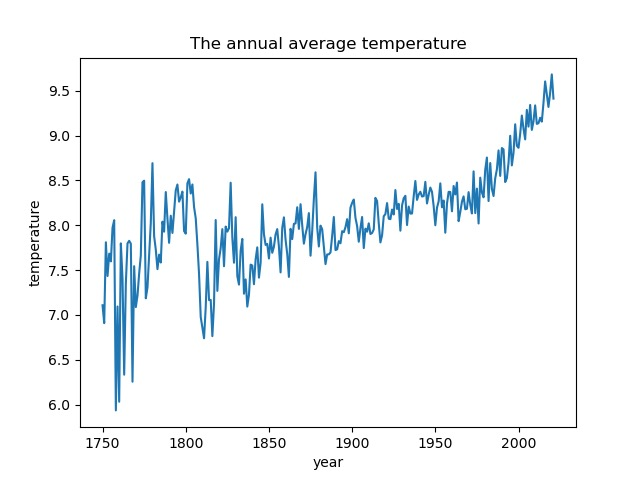
\includegraphics[scale=0.4]{annual avg tem.jpg}
  \caption{picture 1}
\end{figure}

Then we get the average temperature in March between 2011 to 2021 is the following. 

\begin{align*}
  [6.0780,5.9890, 6.2030, 6.3420 , 6.7220 ,7.4750 , 7.1340 , 6.6680 , 7.0950  ,7.0450 ,6.6840].
\end{align*}

\begin{figure}[htbp]
  \centering
  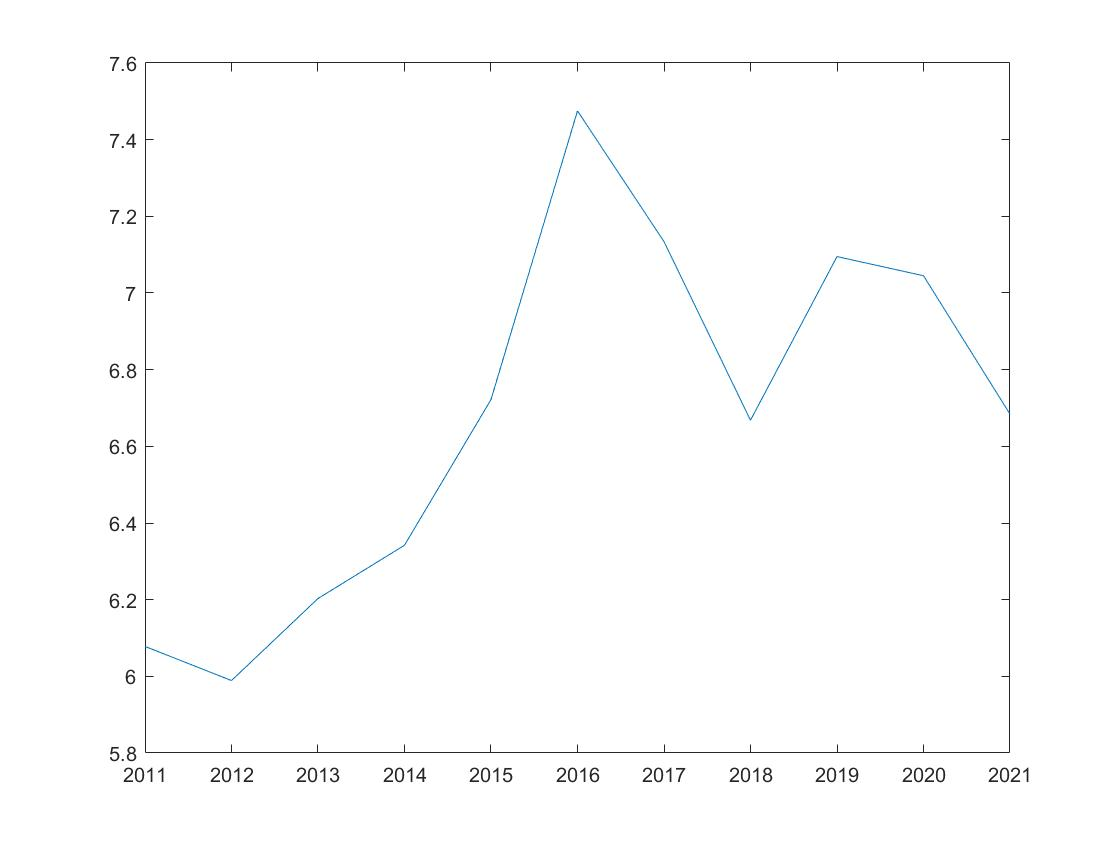
\includegraphics[scale=0.2]{past 10 avg.jpg}
  \caption{picture 2}
\end{figure}

The total increasing rate is 1.100\%, and increase 0.606\oc in value.
Increasing rate respectively is given by
\begin{align*}
  [ -0.0941,-0.0146,0.0357,0.0224,0.0599,0.1120, -0.0456,-0.0653, 0.0640,-0.0070,-0.0512].
\end{align*}
Past 10 years average temperature is 6.6759\oc. 

And the monthly average temperature between January 2022 to October 2022 except March we can calculate is 
\begin{align*}
  [3.989,  4.358, 6.812,9.665, 12.313, 14.742, 15.588, 15.07 ,13.151, 10.811].
\end{align*}
\begin{figure}[htbp]
  \centering
  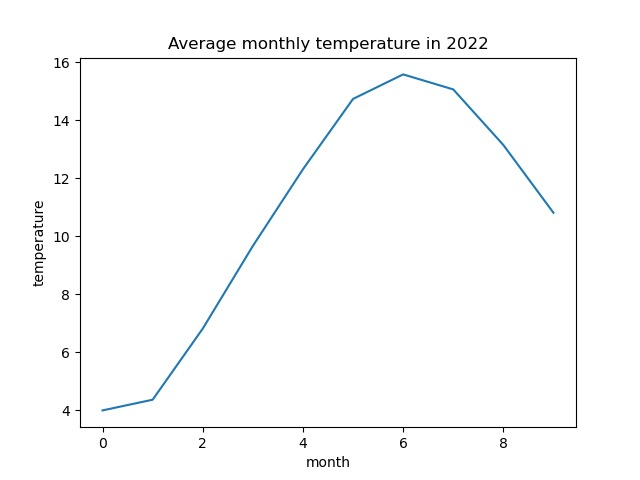
\includegraphics[scale=0.35]{Average monthly temperature in 2022.jpg}
  \caption{picture 3}{fig3}
\end{figure}

Especially, the increasing rate between 2022 to 2021 is 0.0192.
This is much smaller than previous 10 years.


\subsection{(b)}
\subsubsection{Analysis of problem 1(b)}
Question (b) require us to build 2 or more mathematical models to describe the past and predict the future global temperature level.
We can pick a observation as example to analyze the data annually. 
That is we build models using yearly average temperature. 
We decide to use Autoregressive integrated moving average (ARIMA) model and long short term memory algorithm(LSTM) to describe the global temperature.

\subsubsection{Model 1: ARIMA}

ARIMA model, differential integrated moving average autoregression model, also known as integrated moving average autoregression model, 
is one of the time series prediction and analysis methods.
In ARIMA (p, d, q), AR is `autoregressive', and p is the number of autoregressive terms; 
MA is the `moving average', q is the number of moving average terms, and d is the number of differences (orders) made to make it a stationary sequence.
This model is built to describe the relationship between current value and historical value using the historical time data of the variable itself to predict itself.
So it fit to the question in 1(b).

Firstly, we need to determine the order p which means the lagged order i.e how many previous variable related to the current value.
This leads an autoregressive model(AR):
\begin{align*}
  y_t = \mu + \sum^p_{i=1} \gamma_i y_{t-i} + \epsilon_t
\end{align*}
where $y_t$ is current value, $\mu$ is constant.

Then we consider more about the error along the time series. 
We get the moving average model(MA):
\begin{align*}
  y_t = \mu + \sum^q_{i=1} \theta_i \epsilon_{t_i} + \epsilon_t
\end{align*}
This can reduce the random fluctuation when estimating. 

Finally, we combine previous 2 models then obtain the model ARMA
\begin{align*}
  y_t = \mu + \sum^p_{i=1} \gamma_i y_{t-i}  + \sum^q_{i=1} \theta_i \epsilon_{t_i} + \epsilon_t
\end{align*}

But this model has some limitations.
The results that ARMA obtains might not be stationary, then some test will not be credible. 
So we can add a difference order d to let them be stationary. 

We load the dataset `land year std data'

Before we obtain the expression of ARIMA, we need to determine the value of p, q and d.
In general, we choose low value of d i.e low order for the model. 
So it is important to find a reasonable value of p, q.
We can check the Akaike information criterion(AIC) and Schwarz criterion(SC) 
given by respectively:
\begin{align*}
  AIC&=\ln(\frac{SSE}{T})+\frac{2K}{T},\;\;\;\;K=p+q+2.\\
  SC&=\ln(\frac{SSE}{T})+\frac{K\ln(T)}{T}.
\end{align*}
If AIC and SC are small enough, then the choices of p and q are preferred.
So we can use the force algorithm to find the best combination of p, q.

Moreover we need to check which model we should use to estimate the data.
We can check the autocorrelation function(ACF):
\begin{align*}
  ACF(k)=\rho_k = \frac{Cov(y_t,y_{t-k})}{Var(y_t)}.
\end{align*}
k is the lagged index.

We calculate the statistic ACF and plot a scatter so that we can really determine which model is the better one.

After we get the annual average temperature, we first perform a stationarity check on the data. The most intuitive way is to use the data to make a sequence diagram and then observe the trend of the image. At the same time, we calculate the first-order difference and the second-order difference of the data and make a graph to observe the trend.

\begin{figure}[htbp]
  \centering
  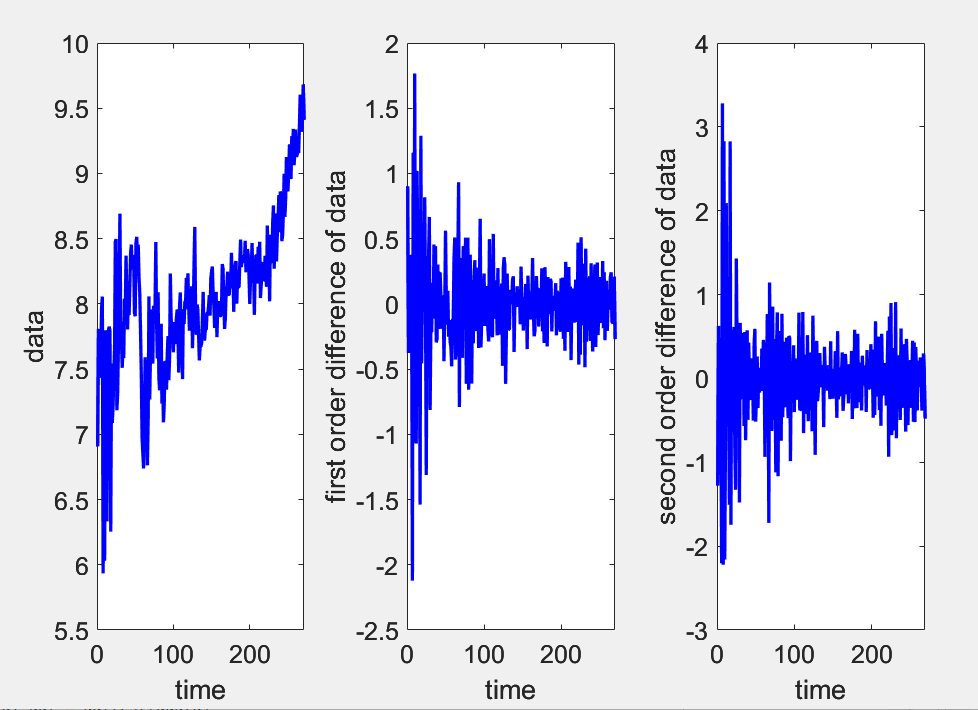
\includegraphics[scale=0.35]{Smoothness Analysis.png}
  \caption{picture 4}
\end{figure}

It is not obvious from the image to confirm the stationary relationship of the data, so we use the mathematical test method——ADF test and KPSS test.

In the ADF test, if the return value is 0, the data is not stationary, and if the return value is 1, the data is stationary. Then in KPSS test, if the return value is 0, the data is stationary, and if the return value is 1, the data is not stationary.

From the test result we can know the raw data is not stationary, so we need to calculate the first order difference of data, then we do the same test to the first order difference of data. We can get
\begin{figure}[htbp]
  \begin{minipage}[t]{0.45\linewidth}
    \centering
    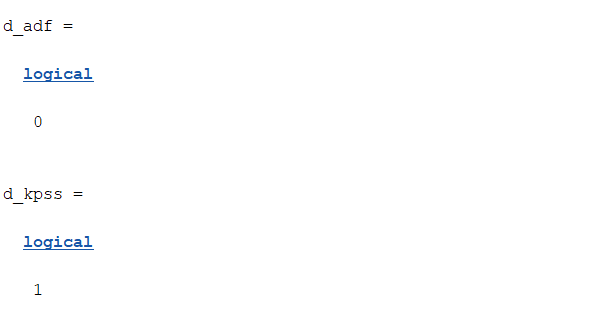
\includegraphics[scale=0.5]{order 1.png}
    \caption{picture 5}
  \end{minipage}%
  \begin{minipage}[t]{0.45\linewidth}
    \centering
    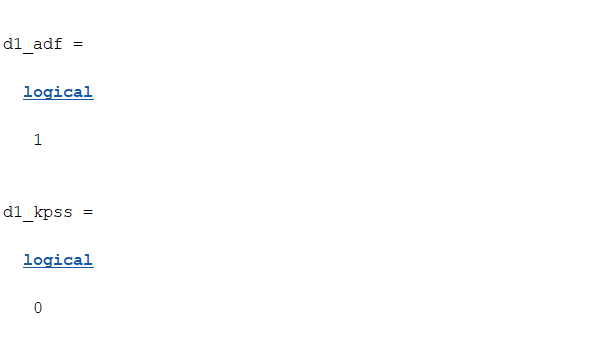
\includegraphics[scale=0.5]{order 2.png}
    \caption{picture 6}
  \end{minipage}
\end{figure}

Therefore, the data after the first order difference can be used for time series modeling analysis. And then what we need to do is to confirm the parameters (p, q, d). The first step is to examine the autocorrelation and partial autocorrelation plots of a stationary time series.

\begin{figure}[htbp]
  \centering
  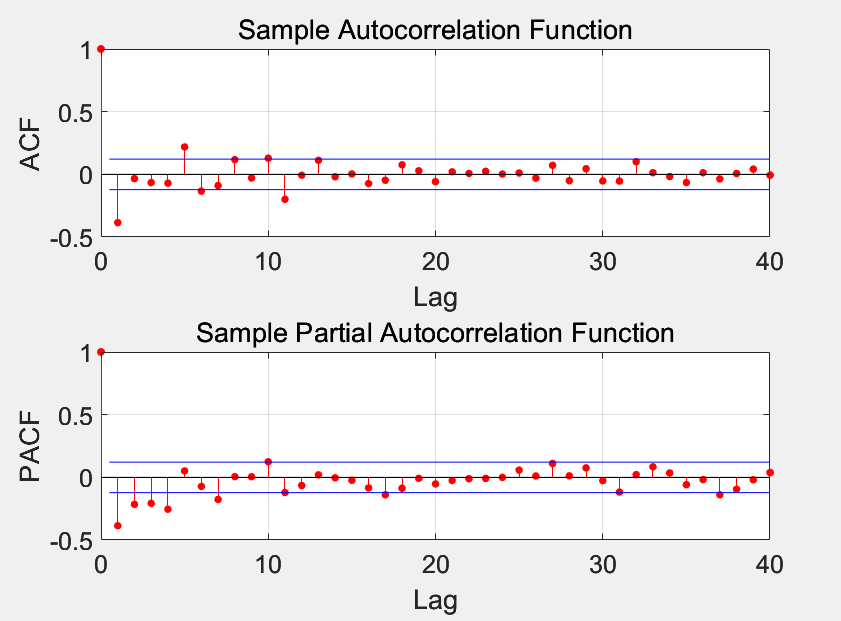
\includegraphics[scale=0.4]{ACF.png}
  \caption{picture 7}
\end{figure}

We can't get the values of p and q from the figure, so we adopt the AIC and BIC criteria to find the most suitable p and q values within a certain range. When we have confirmed the appropriate (p, q, d) value, we can build a model to predict the subsequent data. In the process of forecasting, we also set the upper and lower forecast limits under the 95\% confidence interval.

Finally we get that the best combination of p, q is:
\begin{align*}
  p=3,\;\;q=2
\end{align*}

\subsubsection{Model 2: LSTM}

The recurrent neural network has memory, parameter sharing and Turing completeness, so it has certain accuracy and advantages to select the recurrent neural network for learning and prediction.

LSTM, a short - and long-term memory network, is used in this paper. LSTM is formed by a chain of repeated modules, each of which is called a cell (cell).

Each cell has a specific gate structure to achieve selective information transmission. Through the transmission of LSTM gate structure (forgetting gate, input gate, cell state update, output gate) information, each cell state is updated.

The function of Amnesia Gate is to selectively update the cell state. The first step of LSTM is to determine the cell status update.

It uses the Sigmoid function to $h_{t-1} $and $x_t $ processing, outputting numbers between 0-1. 
1 means completely reserved, while 0 means completely forgotten. Where $h_{t-1} $ is the weight matrix, $b_f$ is the offset term.

\begin{align*}
  f_t = \sigma (W_f \cdot [h_{t-1},\; x_t] + b_f)
\end{align*}

The function of the input gate is to input data and determine the information stored in the cell state.
This part is divided into two steps. First, the Sigmaid layer determines the weight of the input information in the update, that is, which information needs to be updated.
Next, build a candidate vector $\tilde{C_t}$ through tanh calculation at this time

\begin{align*}
  i_t &= \sigma (W_f \cdot [h_{t-1},\; x_t] + b_f)\\
  \tilde{C_t}&= tanh(W_c \cdot [h_{t-1},\; x_t] + b_c)
\end{align*}

Next update the previous cell status $C_{t-1}$, add this matrix and the last cell state after the forgetting gate processing to form $C_t$.
Multiply the previous state matrix by $f_t$, representing selective memory of the last cell state.
Then we add $i_t\cdot \tilde{C_t} $ to the value we get  , the new cell state $C_t$ is obtained.

\begin{align*}
  C_t = f_t \cdot C_{t-1} + i_t \cdot \tilde{C_t}
\end{align*}

Finally, the output gate will output based on the current cell state, passing the current input data through the Sigmaid layer.
Then pass the current cell state through the tanh layer, normalize the matrix between -1 and 1, and perform the basic product operation with the output of the sigmoid layer,
So far, the data of the output part has been determined.

\begin{align*}
  o_t &= \sigma (W_f \cdot [h_{t-1},\; x_t] + b_o)\\
  h_t &= o_t \cdot tanh (C_t)
\end{align*}

Through the module chain network composed of LSTM cell units,
Be able to predict the future through continuous learning of input data.

We set the train set, test set as 2:8.
And predict future 2000 years global temperature.


\subsection{(c)}

According to the model in question 1(b), we can easily predict global temperatures in 2050 and 2100 respectively using different models. 
Moreover we need to find when the average temperature of observation points in ous prediction models will reach 20.00\oc.

\subsubsection{Result from model ARIMA}

First, let's predict the annual average temperature for the next 100 years.

\begin{figure}[htbp]
  \centering
  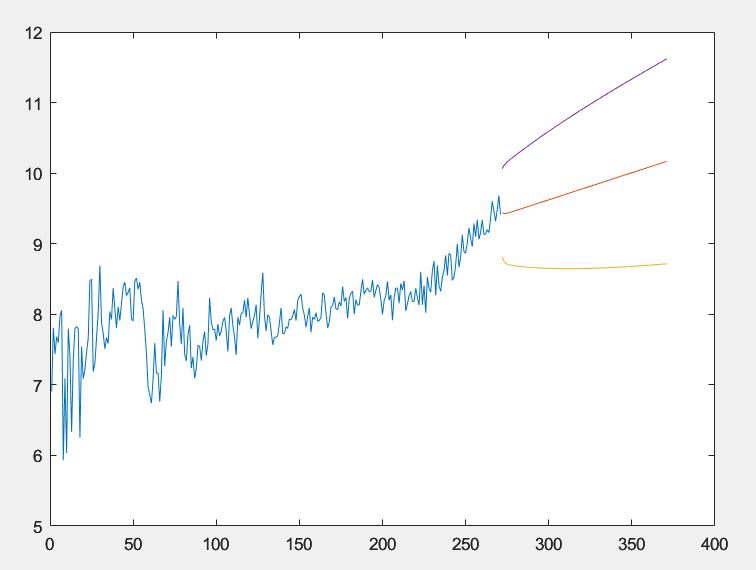
\includegraphics[scale=0.45]{ARIMA prediction 100.png}
  \caption{picture 8}
\end{figure}

\begin{figure}[htbp]
  \centering
  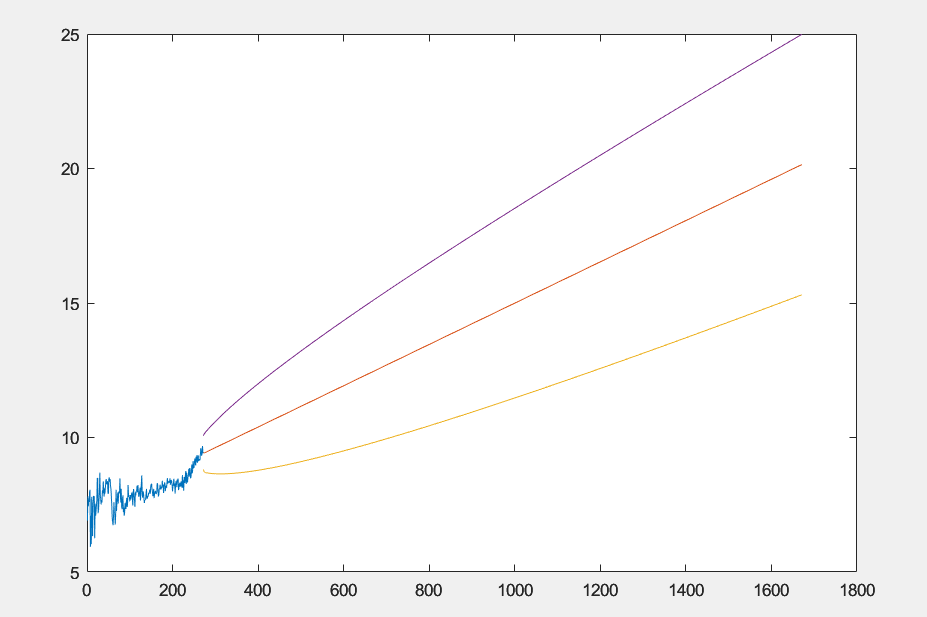
\includegraphics[scale=0.4]{ARIMA prediction 1400.png}
  \caption{picture 9}
\end{figure}

From the predicted results, when it comes to 2050, the annual average temperature will reach 9.6147 \oc. when it comes to 2100, the annual average temperature will reach 9.9985 \oc.

Since 20 \oc has not been reached, we continue to extend the forecast range. We will predict until 1400 years later. We found that when the time comes to 3404 years , the annual average temperature in the world will reach 20.0075 \oc and exceed 20 \oc for the first time.

\subsubsection{Result from model LSTM}

We enter annual standard data into the model, then we predict future 2000 years global temperature.
We draw a picture about the prediction.

\begin{figure}[htbp]
  \centering
  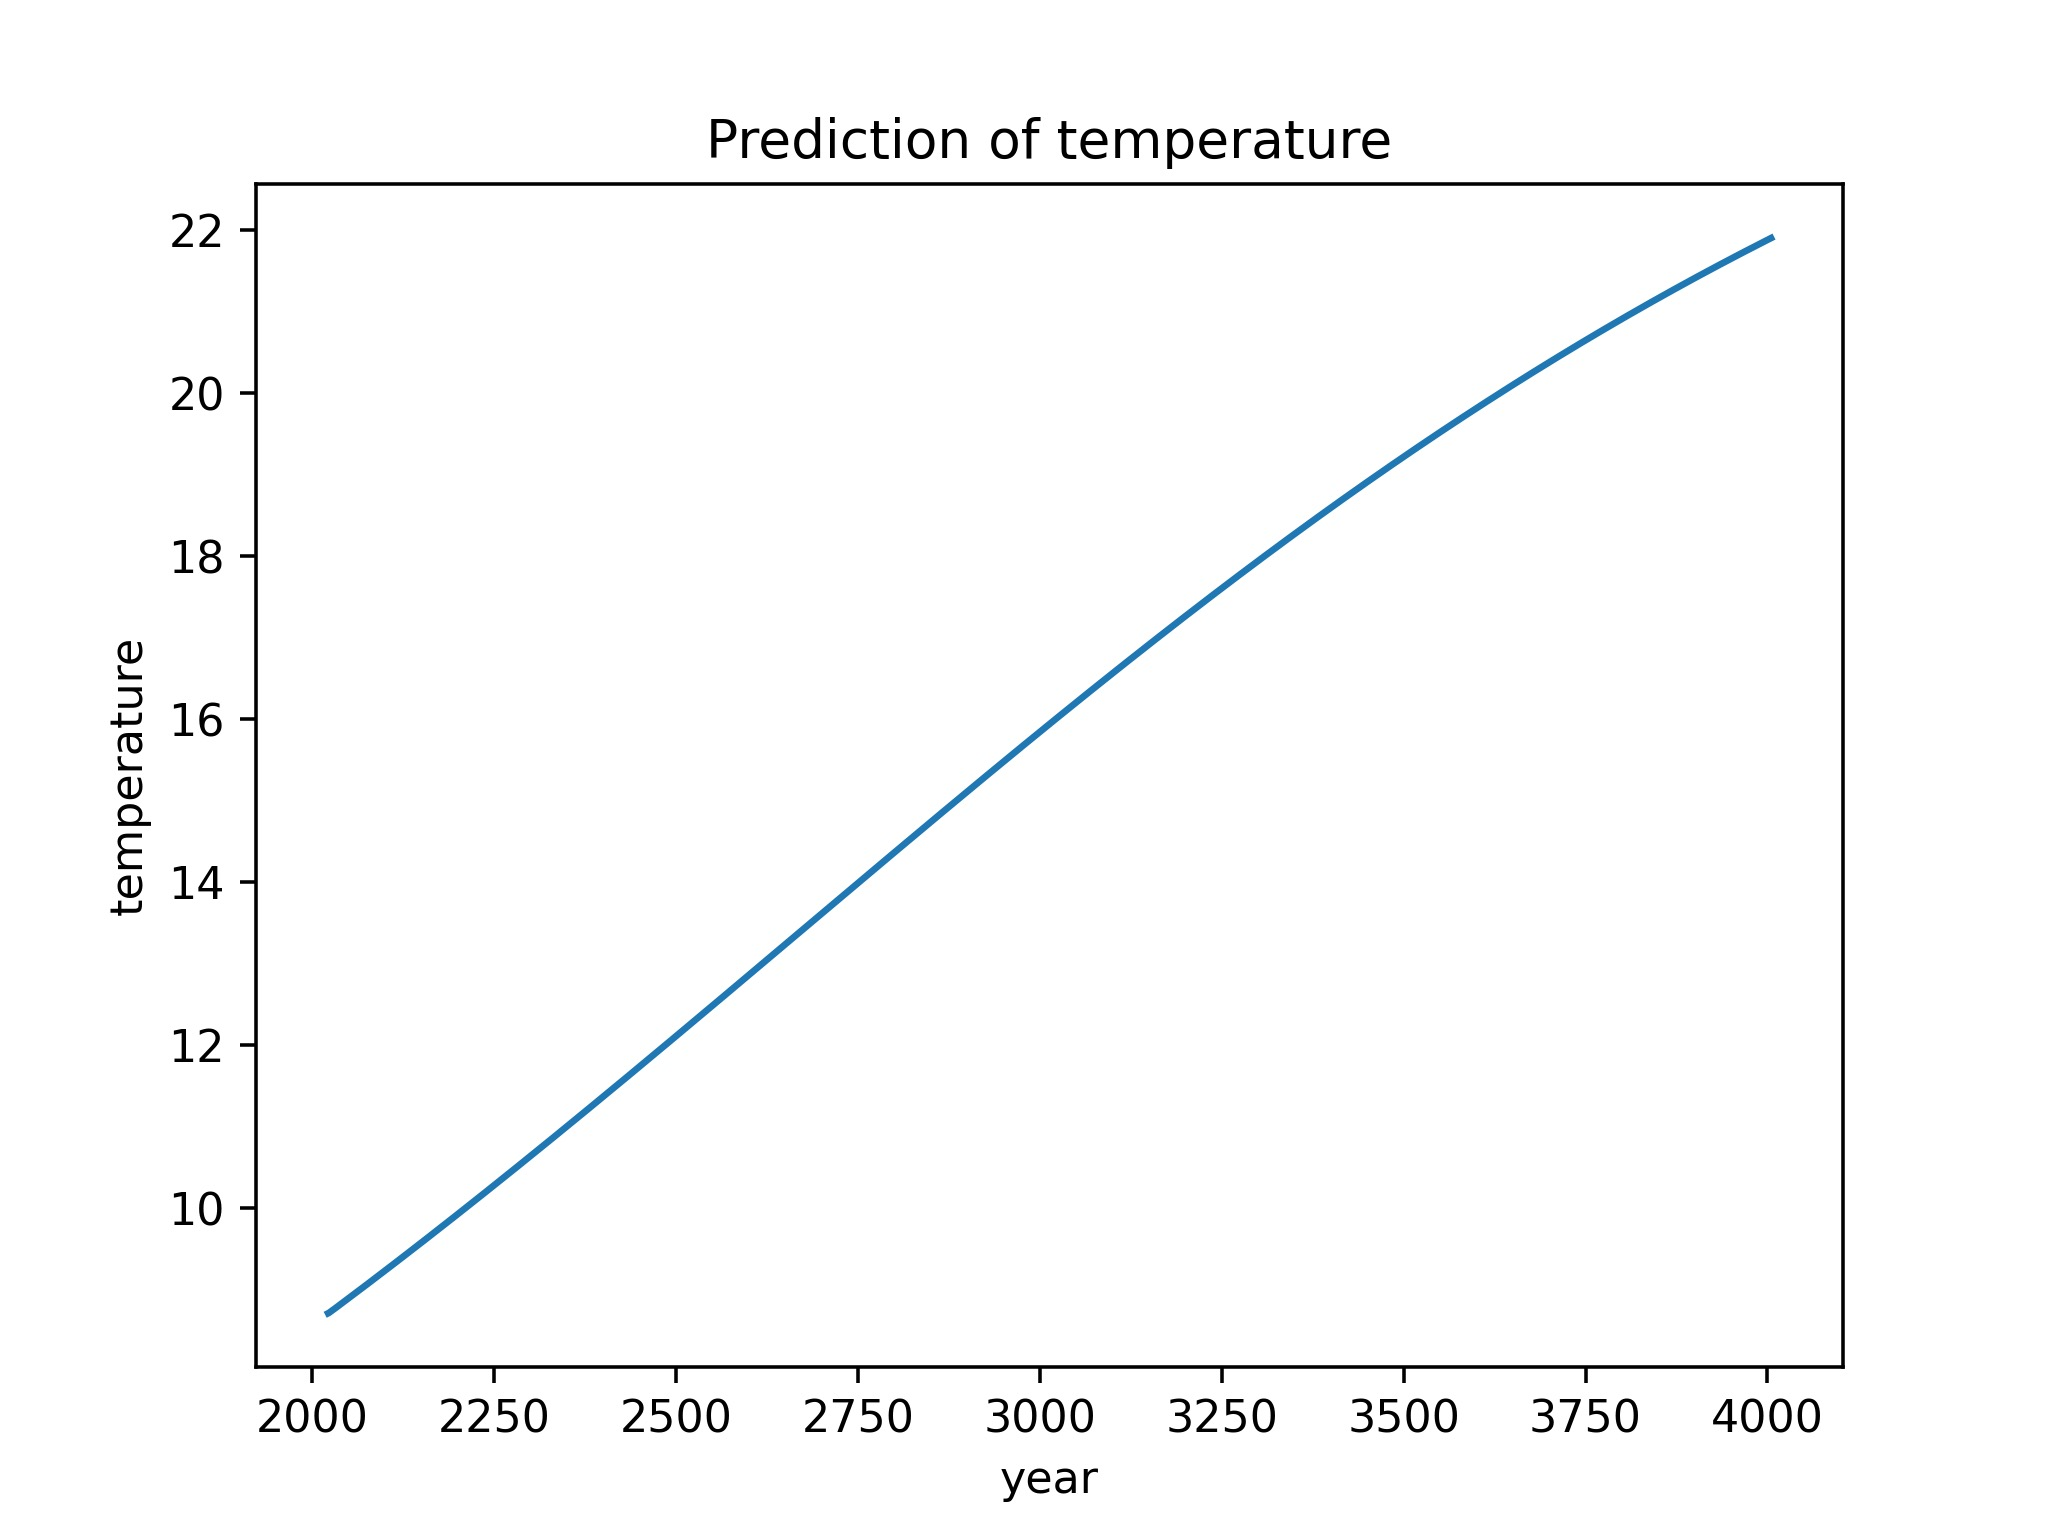
\includegraphics[scale=0.15]{LSTM prediction.jpg}
  \caption{LSTM prediction}
\end{figure}

We can see that, annual global temperature will increase as a line in the future.
We further calculate that in 2050, global temperature will be .
In 2100, global temperature will be .
And finally arrive to 20\oc in 3633.


\subsection{(d)}
We need to calculate important statistics to determine which model is better. 
We compare SE, MSE and RMSE and draw a figure as the following.

\subsubsection{Analysis of model ARIMA}

Using method of statistics, we can get the following analysis of ARIMA(3,2,1).

\begin{center}
\begin{tabular}{c|cccc}
  \hline
   &Value& StandardError& TStatistic &PValue\\
  \hline
  Constant  &  0.0083569    &  0.0052983    &     1.5773    &    0.11473\\
    AR{1}    &    -0.45471   &     0.15899  &        -2.86  &    0.0042368\\
    AR{2}    &    0.27647    &   0.079342   &      3.4845   &  0.00049308\\
    AR{3}    &  0.089483     &    0.0525    &     1.7044    &     0.0883\\
    MA{1}   &     -0.14389   &     0.15508  &     -0.92784  &      0.35349\\
    MA{2}    &    -0.63333   &     0.14147  &      -4.4768  &   7.5784e-06\\
    Variance  &    0.10201   &   0.0054319  &        18.78  &   1.1057e-78\\
  \hline
  \end{tabular}
\end{center}

We can find that, most of the p-values are very small.
So we can conclude that most of the coefficients are reliable except MA{1}.

\subsubsection{Analysis of model LSTM}
In this model LSTM, we calculate the model statistic RMSE.
That is we calculate RMSE as 
\begin{align*}
  RMSE=\sqrt{\frac{1}{N} \sum_{i=1}^n (y_i - f(x_i))^2} 
\end{align*}
where $N=272$, $y_i$ is the real global temperature from 1750 to 2022, and $f(x_i)$ is the prediction of it.
We get $RMSE = 1.792$. 
So we claim that the prediction using LSTM has less reliability than model ARIMA.

In conclusion, we finally choose ARIMA to modify the description of past and future global temperature level.
Because we find that ARIMA statistic is more reliable than LSTM statistic.

\section{Solution for question 2}
In question 2, we are required to build a global temperature model not only including the value of temperature 
but also more other reasons such as position, time, volcanic eruptions, forest fires and the COVID-19 etc.

\subsection{(a)}
\subsubsection{Analysis of problem 2(a)}
According to the data given in attachment 1, we analyze the correlation between global temperature, time and location.
We can use multiple regression to describe the relationship between global temperature, time and location. 

\subsubsection{Relationship about location}
We first analyze the relationship between latitude and temperature. 
And we conclude that only latitude effects temperature by geometry.
Since we only consider the relationship between latitude and temperature, so we can arbitary choose data in one year.
We use different observation points to denote different latitude.
Then we can get average temperature in 2010, for example, while every temperature represents different latitude. 
And we draw a heat picture to describe the relationship.

\begin{figure}[htbp]
  \centering
  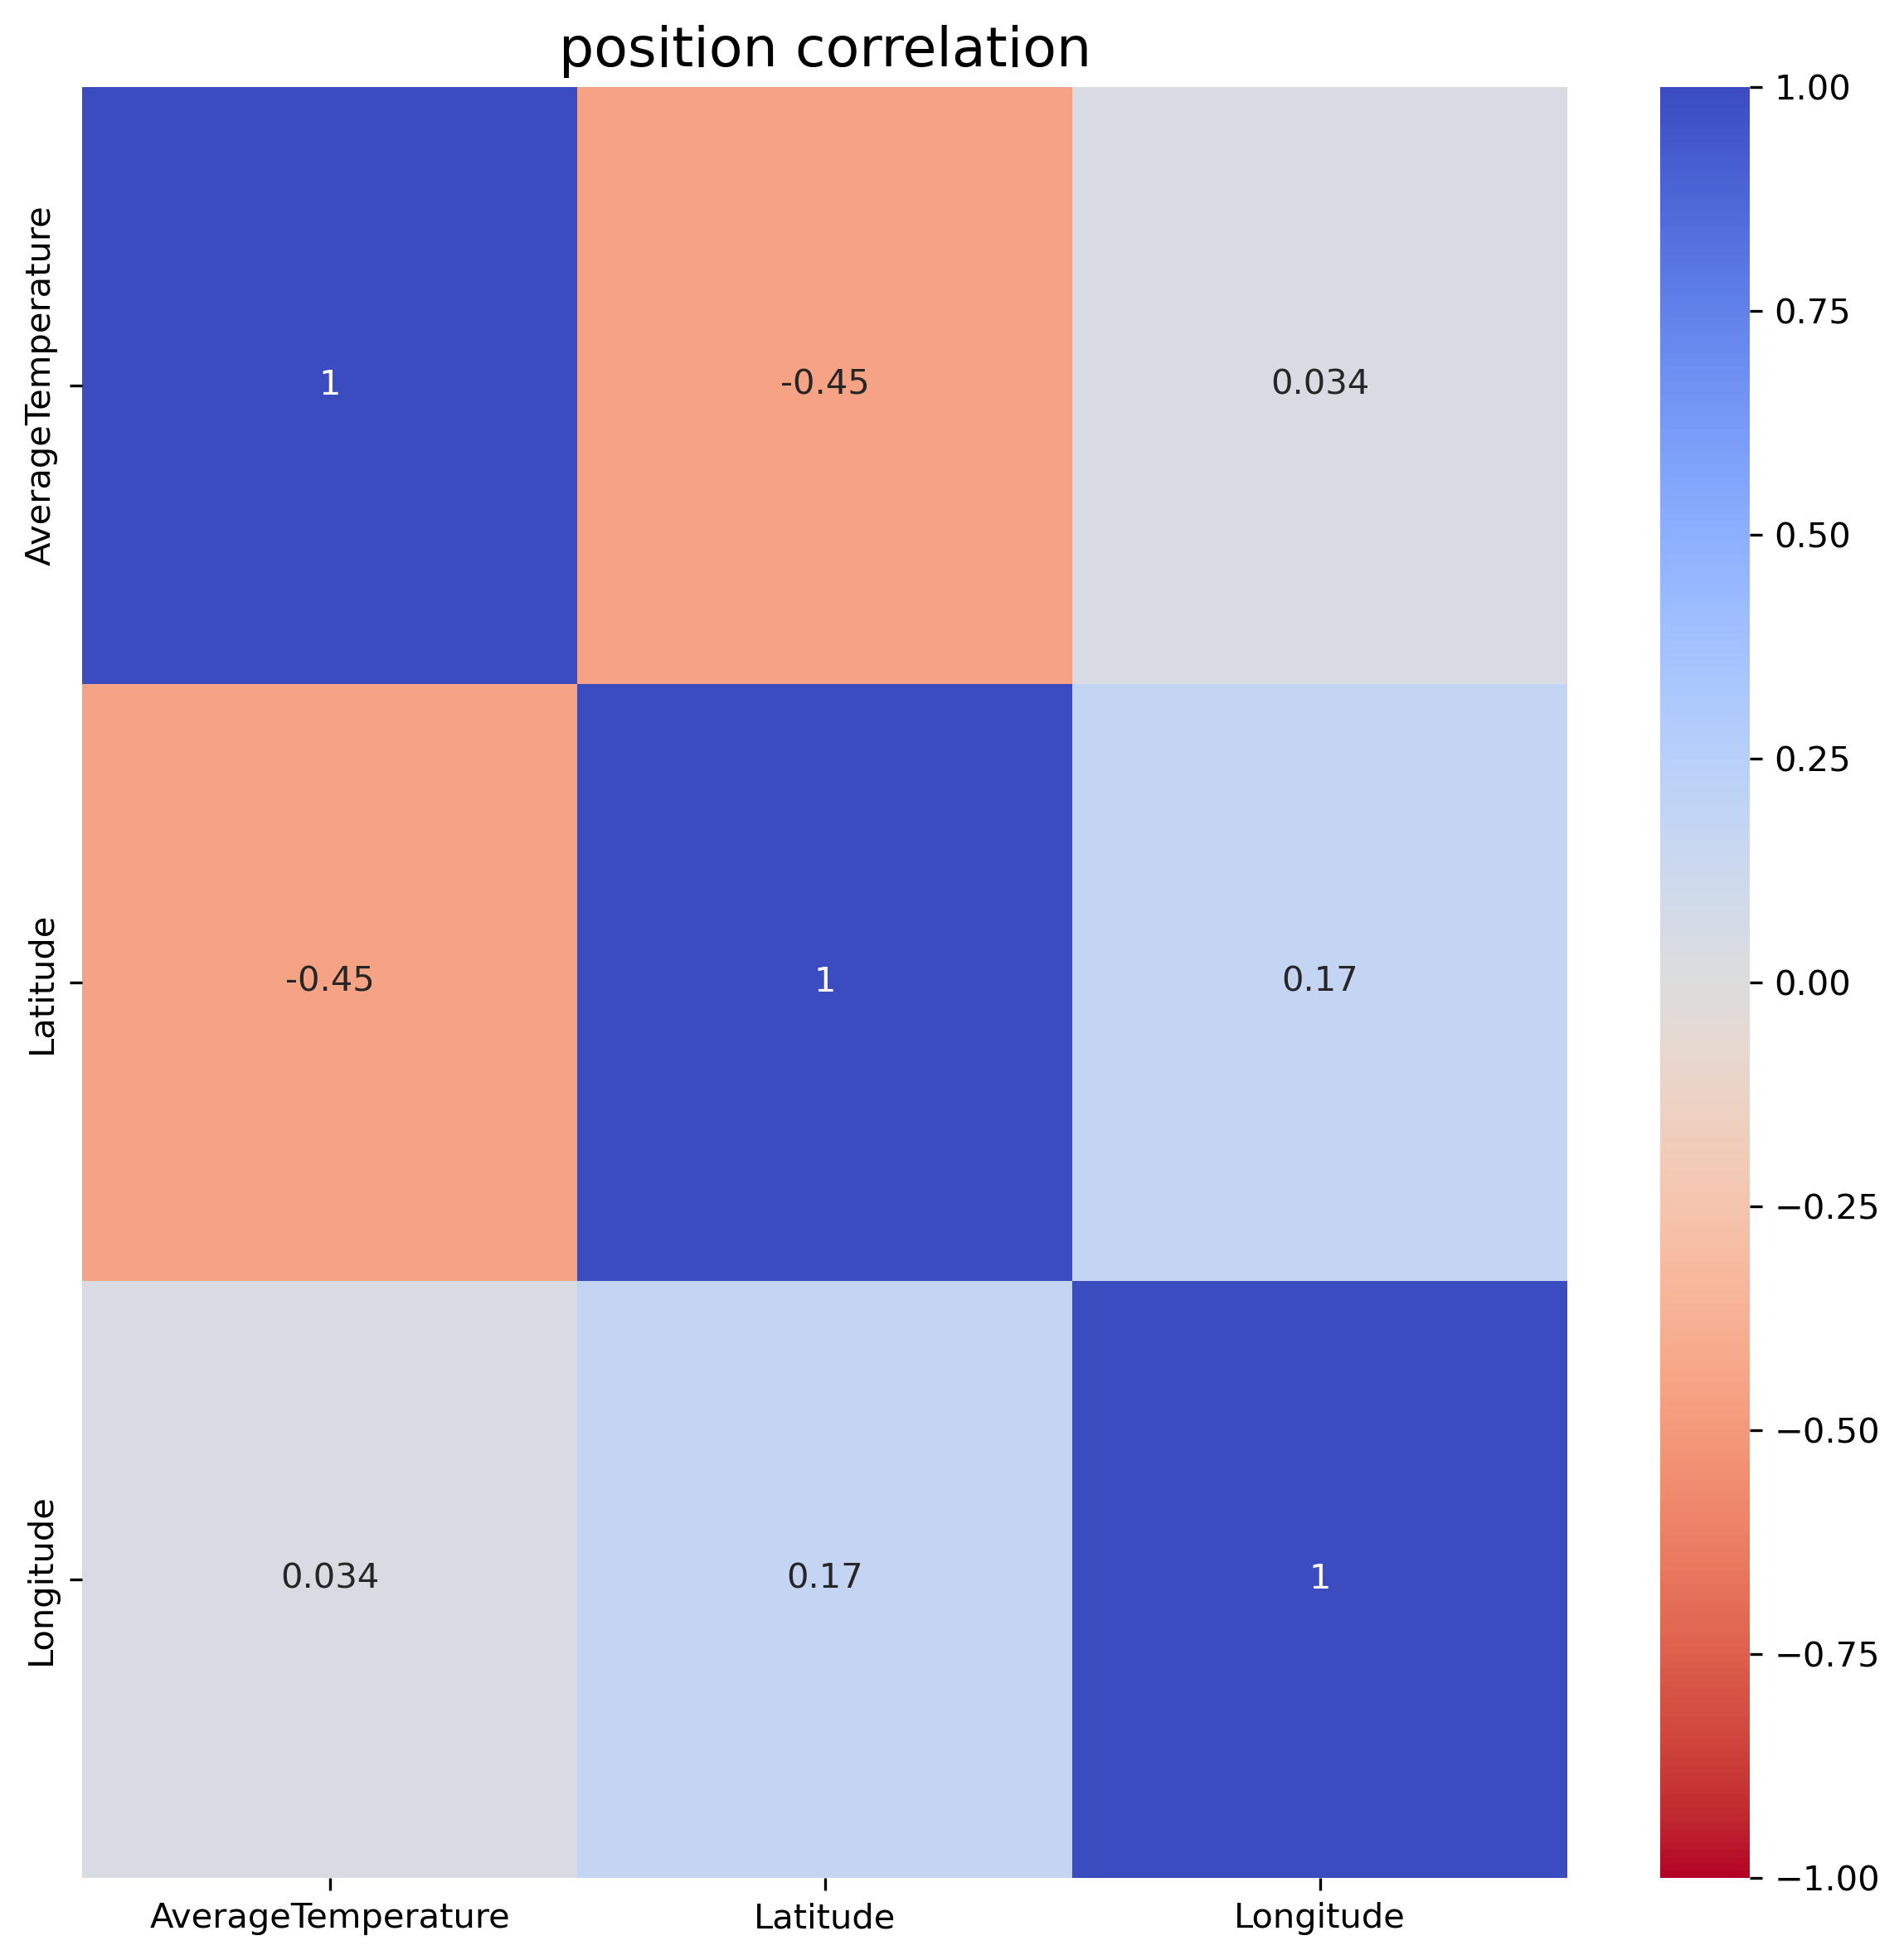
\includegraphics[scale=0.4]{position correlation.png}
  \caption{position correlation}
\end{figure}

Moreover, we make a statistic table for regression model.

\begin{figure}[htbp]
  \centering
  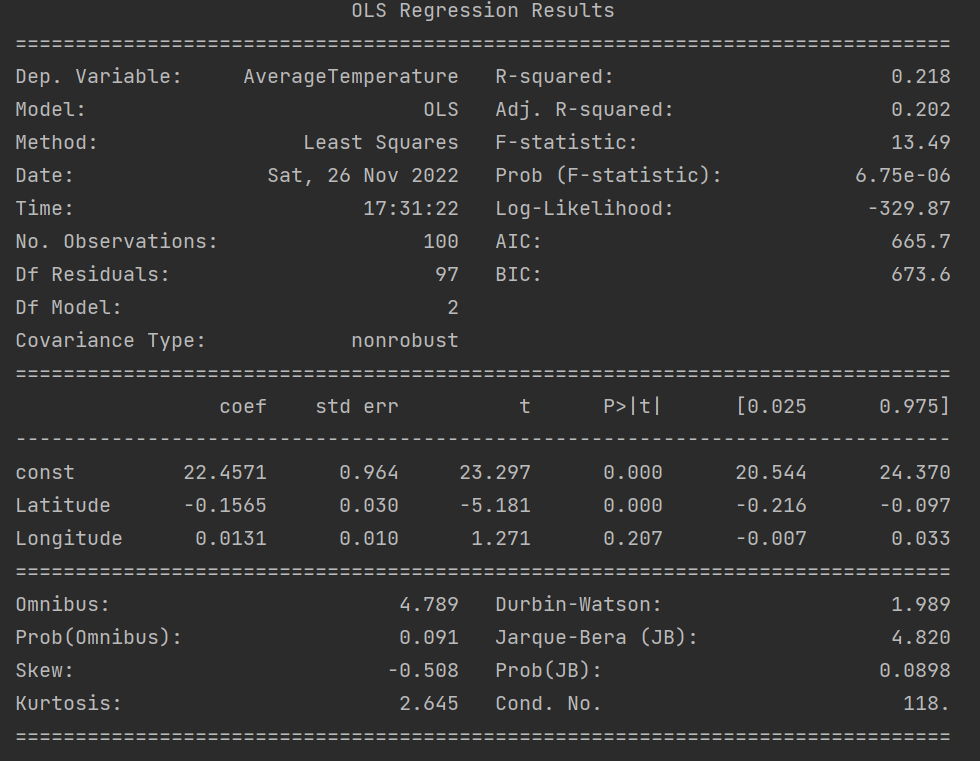
\includegraphics[scale=0.52]{2a table.png}
  \caption{regression table}
\end{figure}

We can see that p-value is small enough, so we can conclude that this model is good.
And we conclude the relationship between temperature and location:
\begin{align*}
  Avgtemperature =-0.1565\cdot latitude+0.0131\cdot longitude + 22.4571.
\end{align*}

\subsubsection{Relationship about time}
Then, we analyze the relationship between global average temperature and time.
We choose one city Shanghai to analyze since we need to reduce the effect of location.
So we pick several years monthly average temperature of Shanghai.
And we divide every year as a period to use the seasonal statsmodel package.

We can get the time series decomposition.

\begin{figure}[htbp]
  \centering
  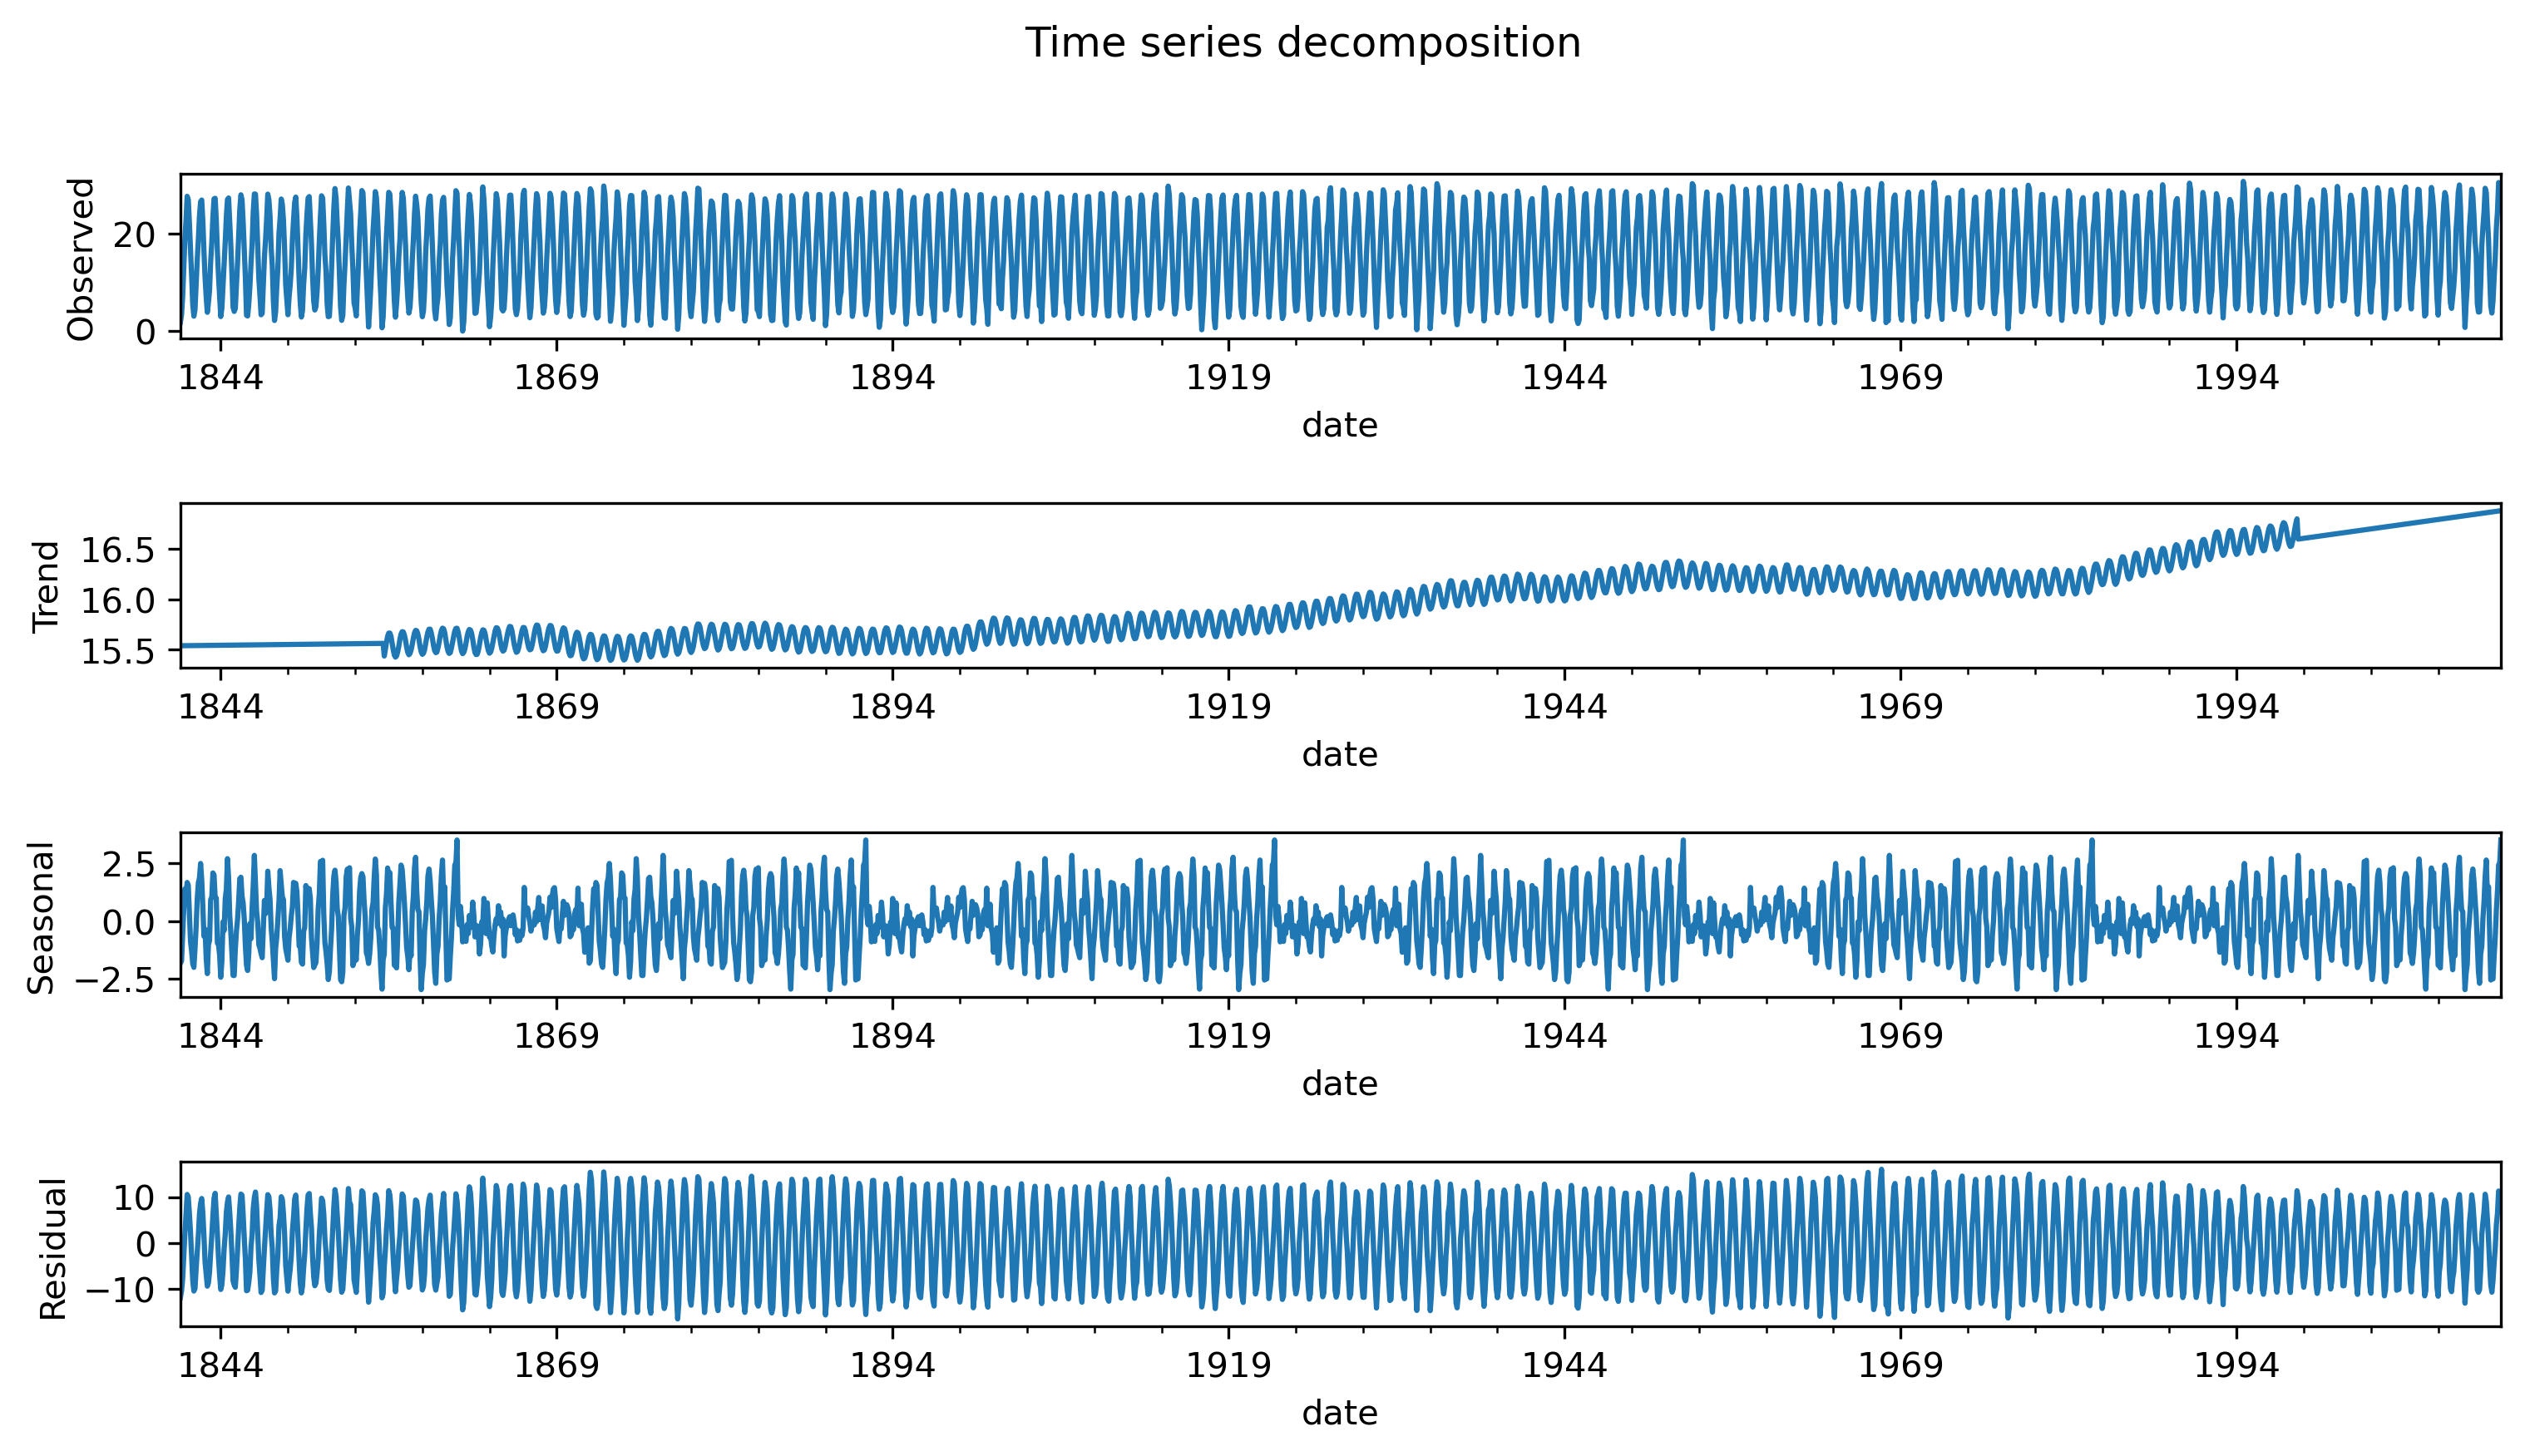
\includegraphics[scale=0.5]{seasonal.png}
  \caption{time series decomposition}
\end{figure}

We find that the estimation and resident are almost stable, and the observed temperature data has very small increasing trend. 
We need to confirm that time has no relationship to global temperature.

Then we use augmented Dickey-Fuller test to judge if time factor is a noise for average temperature.
We get that the p-value is 3.421929753273345e-10.
So we claim that time has no relationship to global temperature.


\subsection{(b)}
In this section, we should get data of the natural disasters, we find part of data(such as volcanic eruptions, forest fires) in \url{https://www.emdat.be/} and part of data(COVID-19) in \url{https://covid19.who.int/data}.

\subsubsection{Relationship analysis}
In this section, we choose 2010 volcanic eruptions in Ayafara, Iceland to analyze the average temperature change of Iceland in 2010.
We plot the average temperature of Iceland from January 2009 to December 2011.

\begin{figure}[htbp]
  \centering
  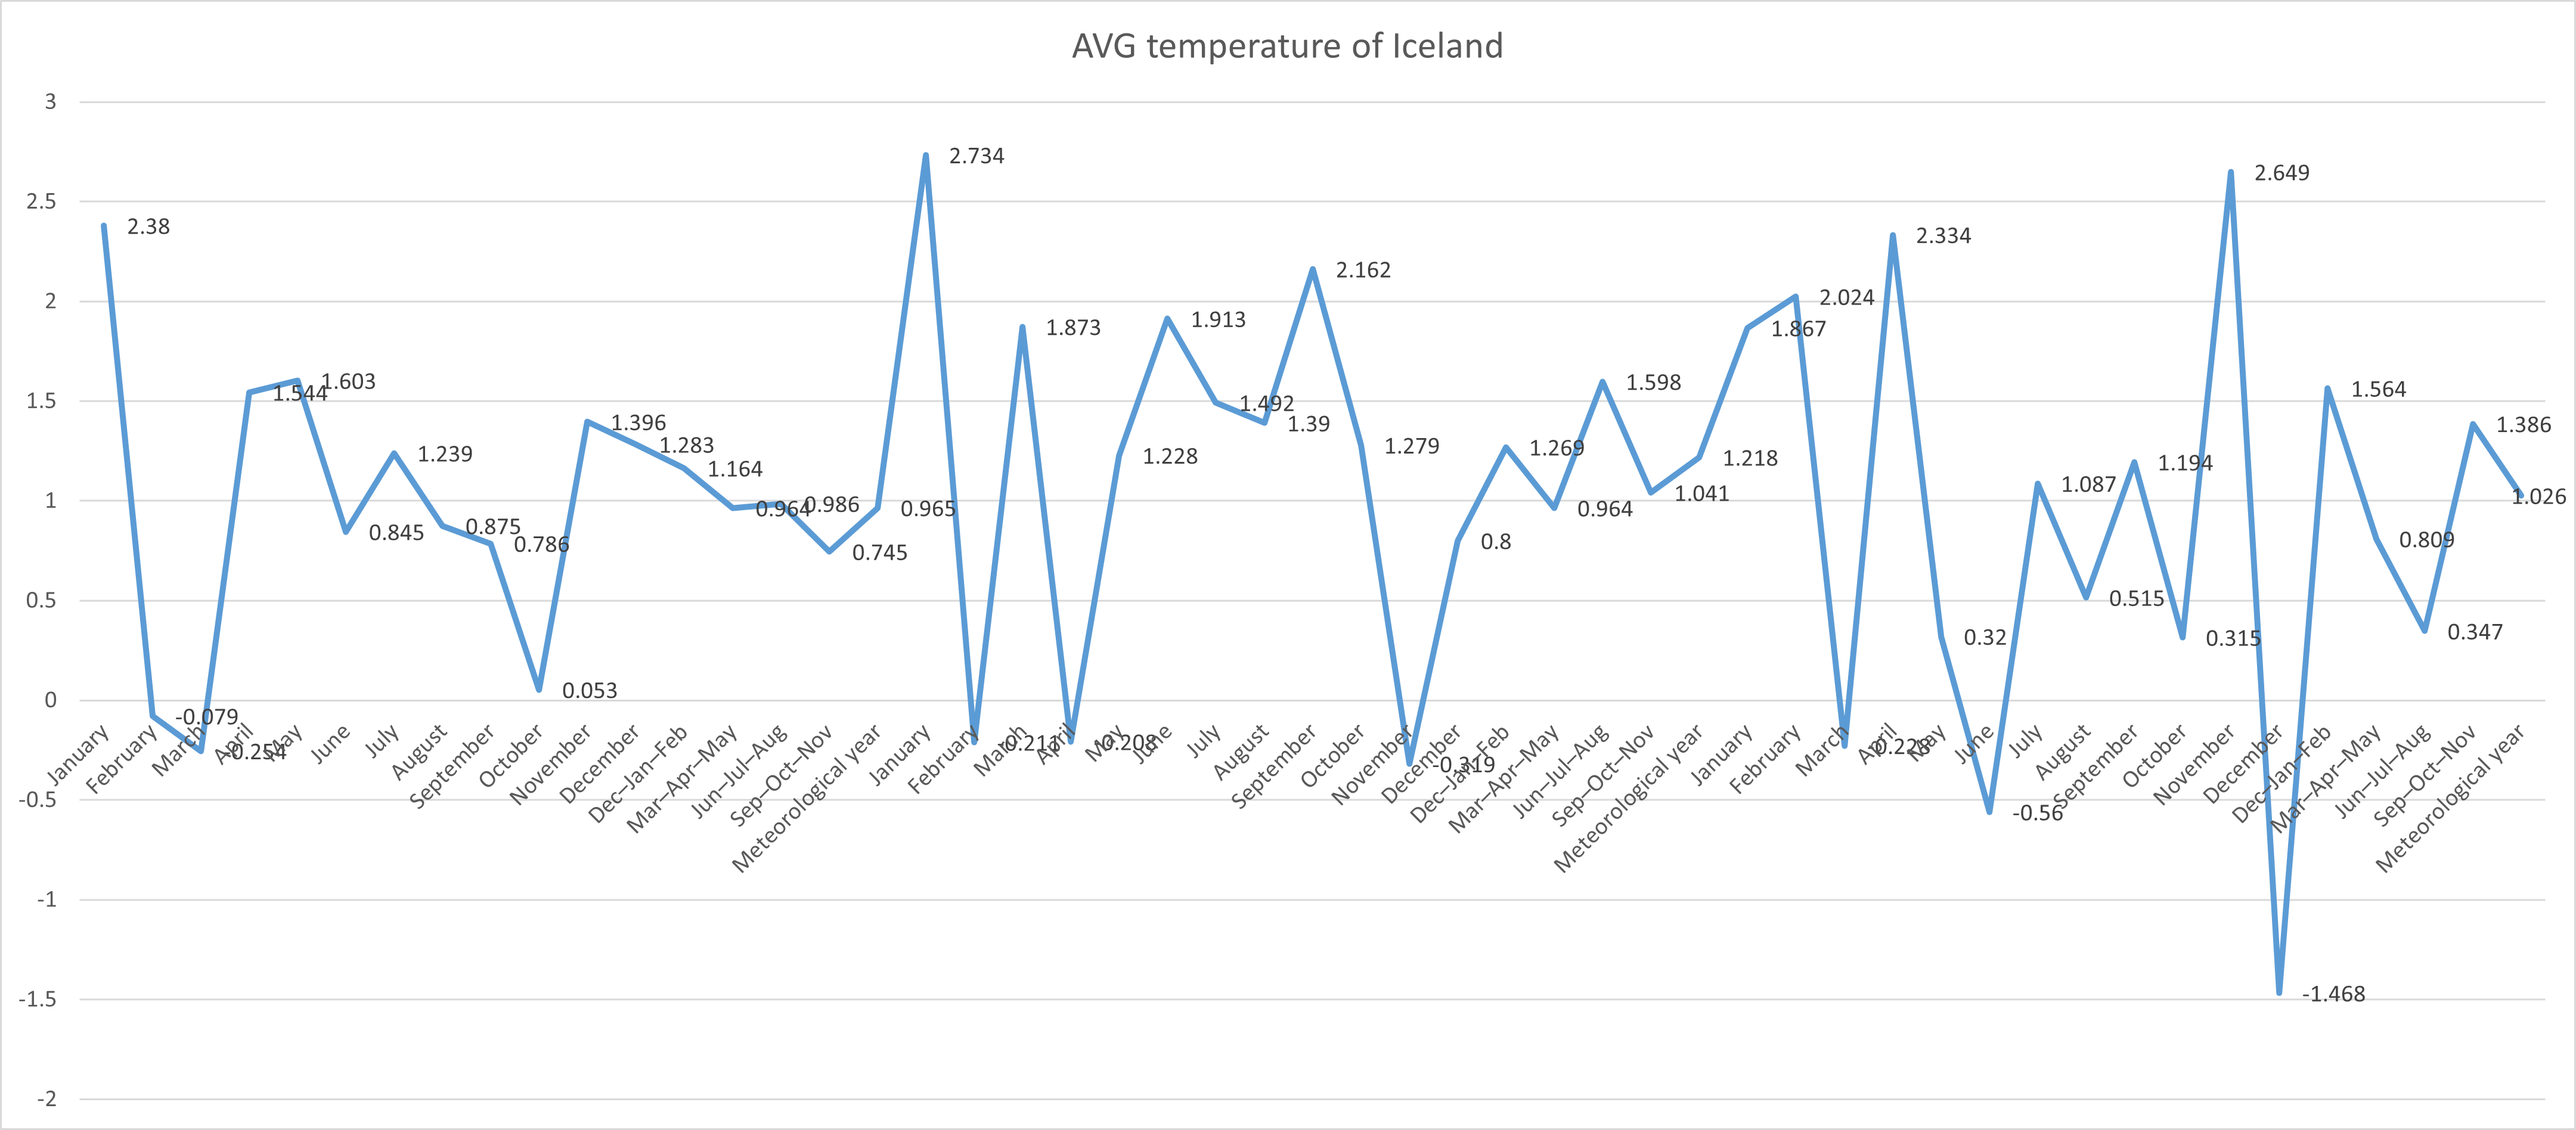
\includegraphics[scale=0.45]{Iceland.png}
  \caption{temperature of Iceland}
\end{figure}

Eyjafjallajokull erupted on 20th March, 2010 first.
Then it erupted on 14th April again.
We want to discover if the eruption affected the local temperature. 

Let's focus on the figure.
We find that the avg temperature in 2010 is different to 2009 and 2011, which has abnormal value in February and March.
The temperature in this two months was on the opposite. 
In March, 2010, the temperature increase to 1.873\oc, while -0.079\oc and -0.228 in 2009 and 2011 respectively.
Moreover, in April, 2010, the temperature was still a abnormal value which was -0.208\oc.
After that, there was a high avg temperature during May to October up to 1.577\oc.
It is 0.677\oc greater than which in 2009, and 1.0985\oc greater than which in 2011.
And the avg temperature 1.577\oc is almost 0.5\oc greater than the annual temperature of Iceland.
It is a very abnormal value for Iceland.
And we claim that there is a positive relationship between volcanic eruptions and global temperature. 

Next, we analyze the relationship between forest and global temperature.
We choose the 2019 Australian forest fires.
The forest fires in 2019 is a major natural disaster. 
And we plot the average temperature of Australia from January 2018 to December 2020.

\begin{figure}[htbp]
  \centering
  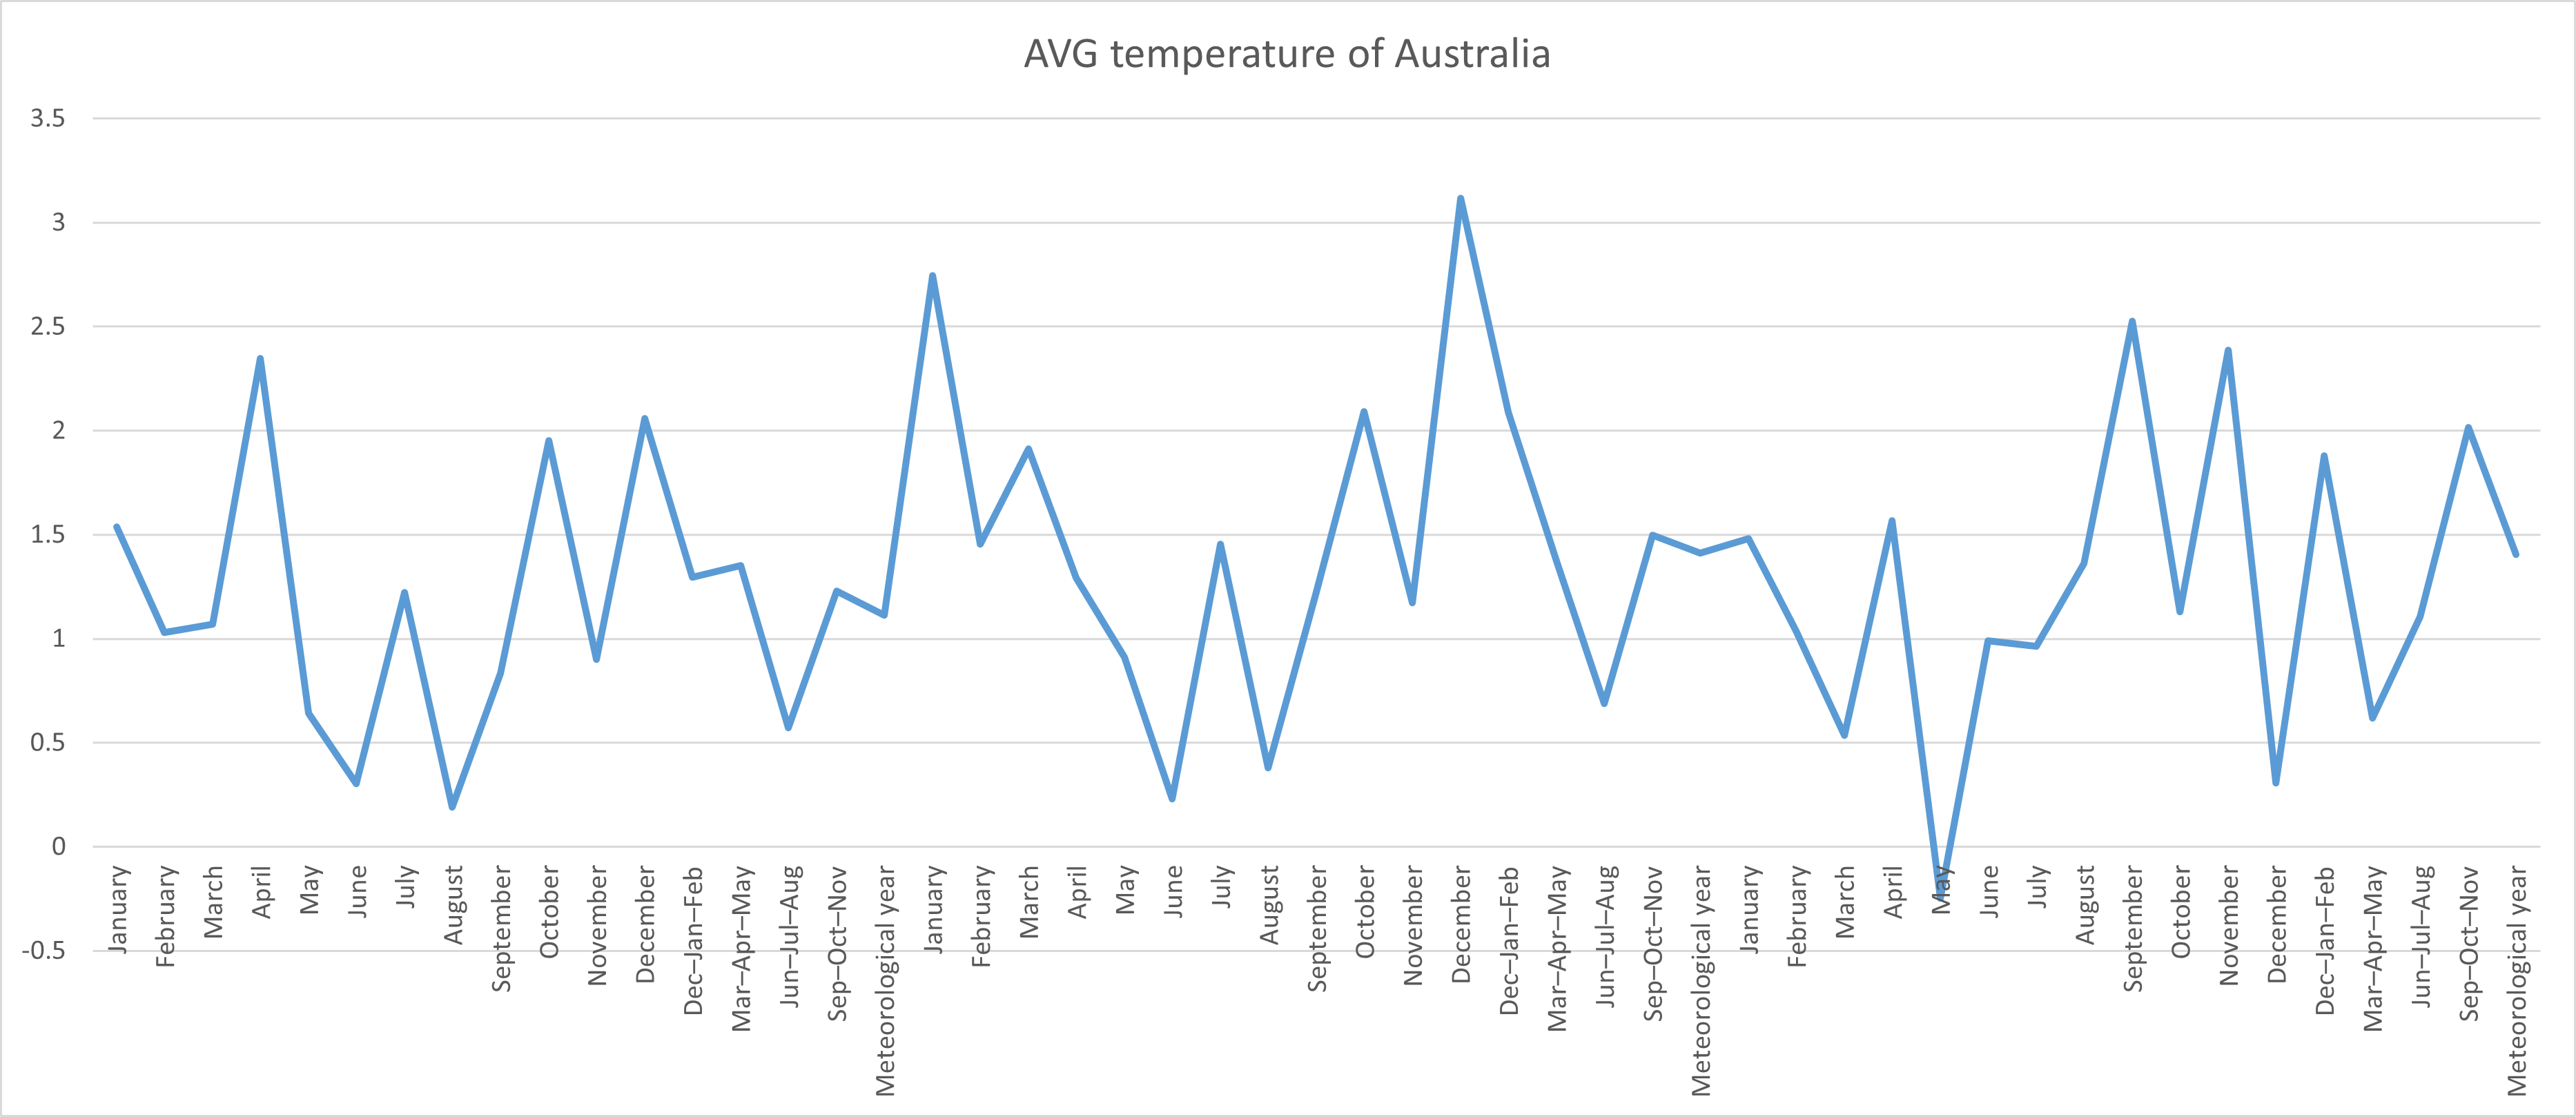
\includegraphics[scale=0.5]{Australia.png}
  \caption{temperature of Australia}
\end{figure}

The Australian forest fires was last for 1 year.
So we focus on July, 2019 to July, 2020.

The avg temperature during the forest fire is 1.268\oc.
And there is 1.093\oc during July, 2018 to July, 2019.
It is 0.175\oc greater.
We claim that there still a positive relationship between forest fires and global temperature.

Last but not least, we consider the relationship between COVID-19 to global temperature.

We can draw the picture about injected number and temperature from 2020 Jan. 

\begin{figure}[htbp]
  \centering
  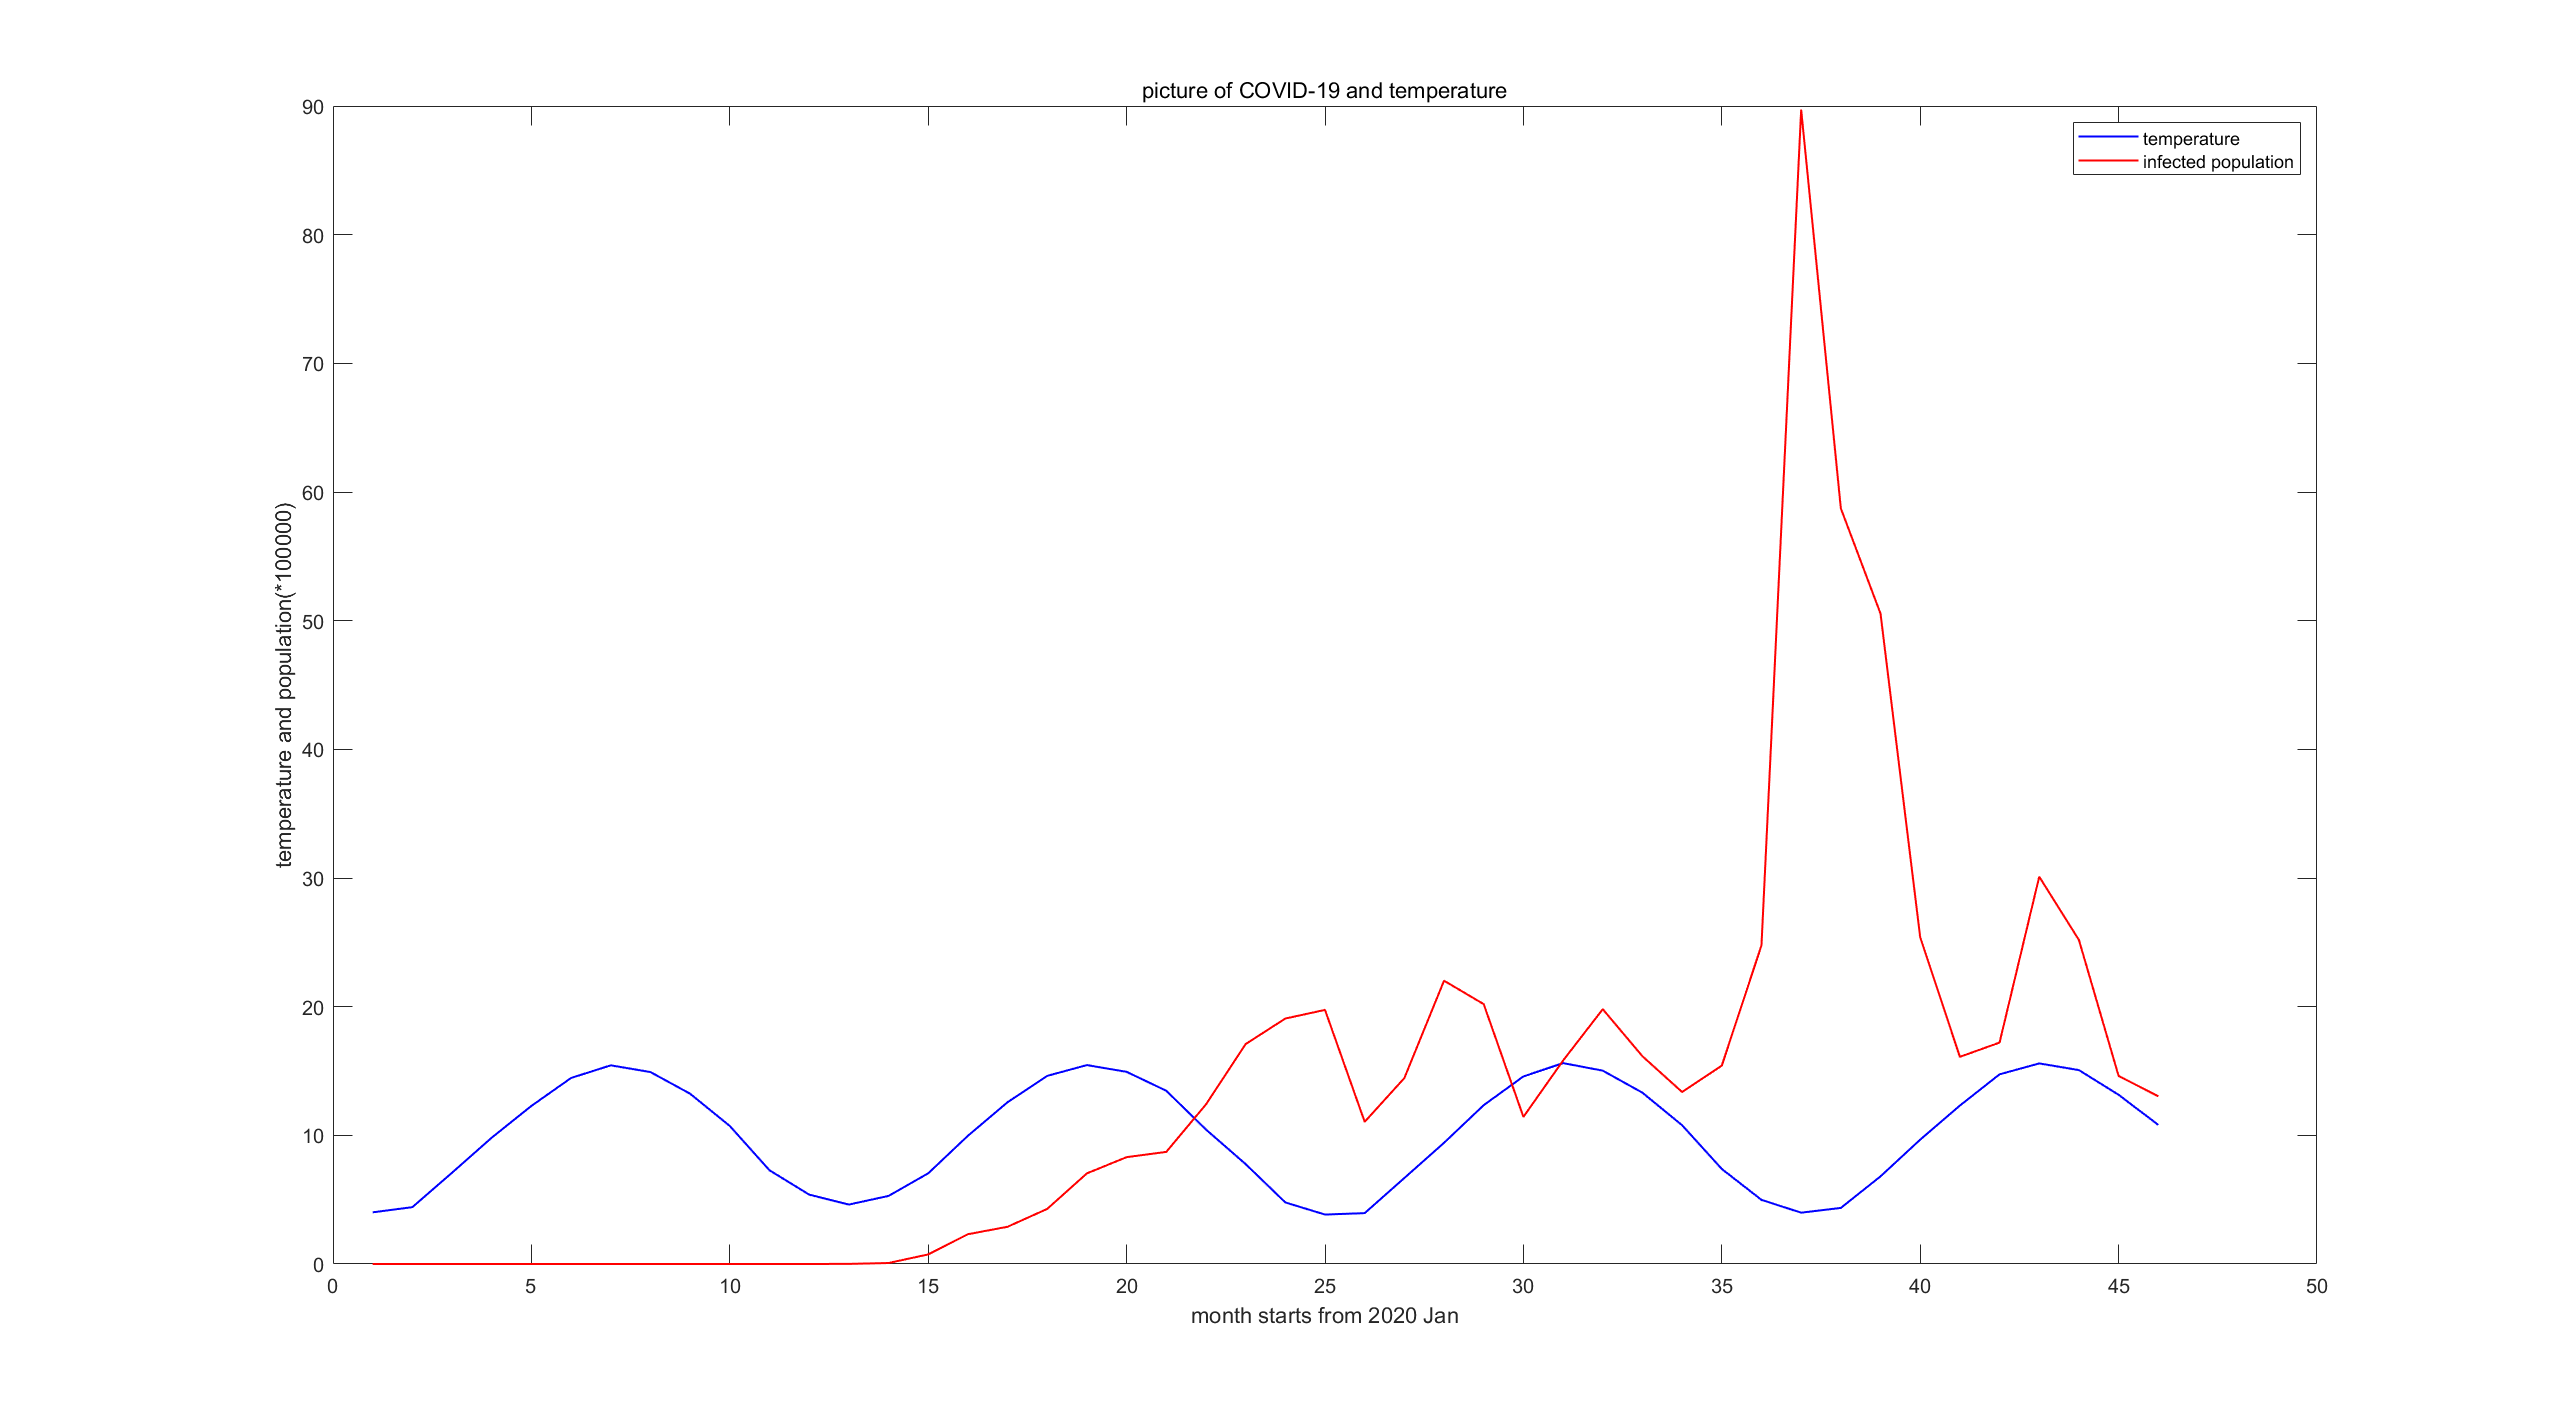
\includegraphics[scale=0.2]{COVID-19.png}
  \caption{COVID-19 and temperature}
\end{figure}

We calculate the average temperature of first 15 months is $avg1=9.0693$,
and $avg2=10.5949$ represents last 31 months when COVID-19 burst. 
We can see that after COVID-19 burst in 2020 Jan, the global average temperature arised about 1.5256\oc.
And this rise is reasonable because people need more activities to fight against COVID-19.
So people around the world will take action such as large transport, factory produce etc. 
In other words, this will lead to entropy increase and be characterized by global average temperature rise.
So we still claim that there is a positive relationship between global temperature and COVID-19.

\subsubsection{Summary}
In question 2(a), we search the relationship betweennatural disasters (such as volcanic eruptions, forest fires and the COVID-19) and global temperature.
And take the example of 2010 Eyjafjallajokull eruption, 2019 Australian forest fires to consider the relationship about local temperature.
Then expand the local conclusion to global conclusion that there is a positive relationship between volcanic eruptions, forest fires and global temperature. 
Moreover, we find that COVID-19 also has a positive relationship to global temperature.

Human activities fighting against this kind of disasters is a vital reason for global warming.
And disasters can also be considered as a entropy increase of the Earth.
They are the global activities that affecting human being.
So people must produce more heat during disasters than other time.
We conclude that disasters make global temperature increase.

\subsection{(c)}
\subsubsection{Data of more factors}
We find datasets of world energy, world population and Global forest resource. \\
\url{https://population.un.org/wpp/Download/Standard/MostUsed/}\\
\url{https://fra-data.fao.org/WO/fra2020/dataDownload/}\\
\url{https://www.gddat.cn/newGlobalWeb/#/FeatureAnalysis}\\
\url{https://www.fao.org/faostat/en/#data}.

\subsubsection{Analysis of relationship}
Then we can use Grey Relation Analysis (GRA) to estimate the relationship between other factors

\subsubsection{Build GRA}

In fact, the GRA algorithm provides a way to measure the distance between two vectors. 
For a time factor, a vector can be considered a time curve, while the GRA algorithm is measured if the shape and trend of the two curves are the same. 
In order to avoid other interference and the effect of protruding morphological features, the GRA first makes normalization, 
fix all vectors in the same size and position, and then calculates the distance of each point. 
Finally, by adjusting min function and max function the last output result falls between 0 and 1, corresponding to the general definition of * * coefficient **. 
Rho fixes the difference between different coefficients of correlation, in other words, the difference in output, t o be harder or more compact. 
From the mathematical point of view, the algorithm measures the sum of the reciprocal $l_1$ norm distance of each dimension of the normalized sub vector and the parent vector, 
and maps it to the 0~1 interval as a strategy to measure the correlation between the sub vector and the parent vector.

\subsubsection{Result from GRA}
Using GRA method, we can get the result is:
\begin{figure}[htbp]
  \centering
  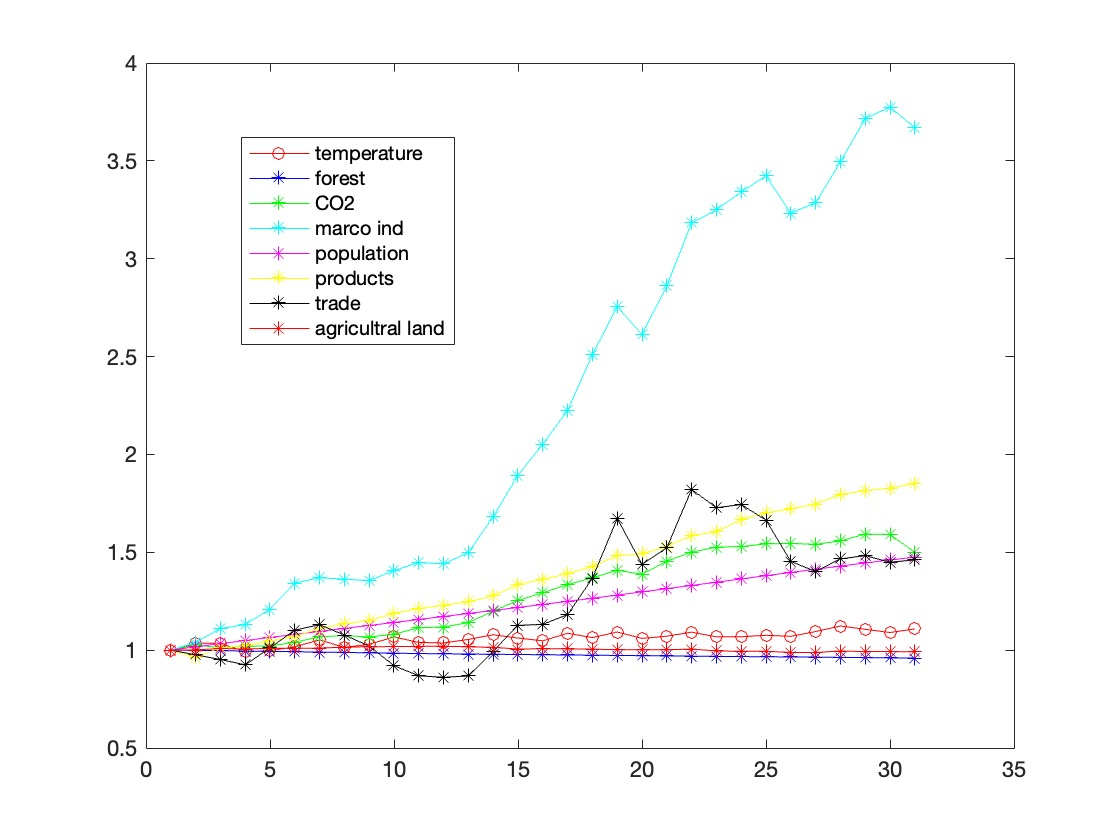
\includegraphics[scale=0.25]{2c1.jpg}
  \caption{Normal data of factors}
\end{figure}

\begin{figure}[htbp]
  \centering
  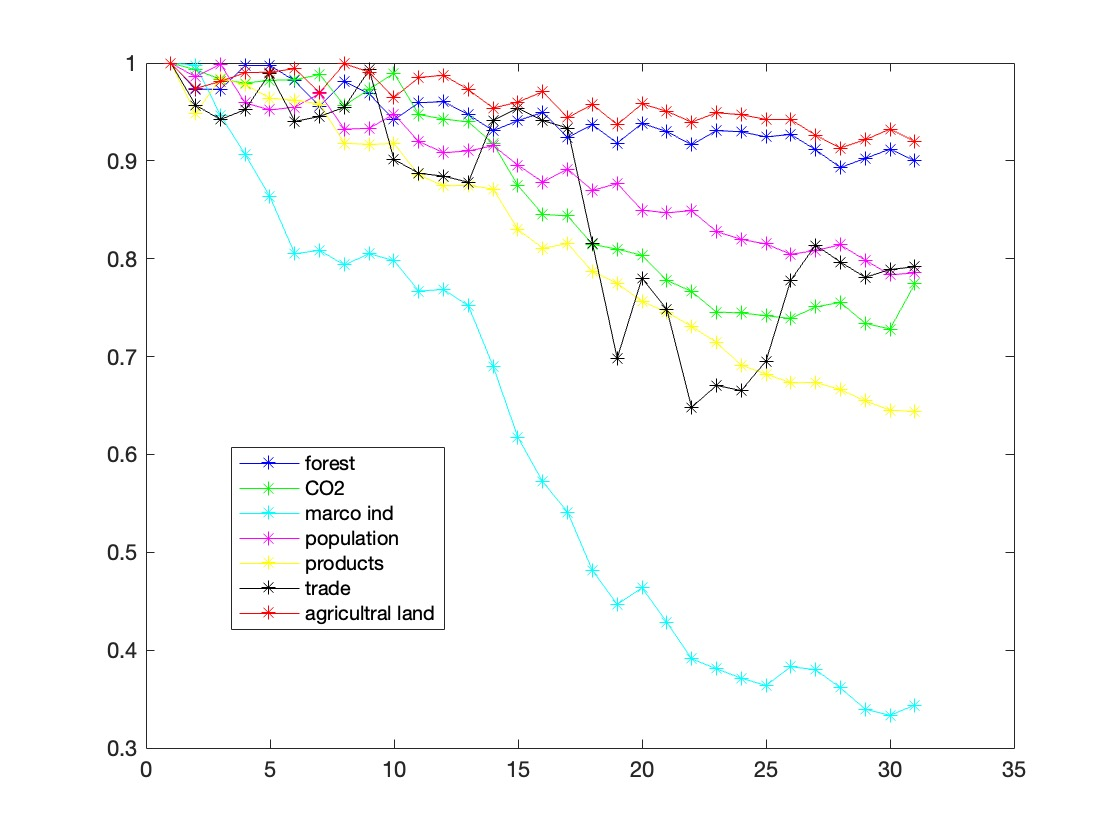
\includegraphics[scale=0.25]{2c2.jpg}
  \caption{Normal data of factors}
\end{figure}

By using the additional 7 types of data collected, we use GRA(Grey Relation Analysis) to establish an evaluation system to determine which indicators have the greatest impact on temperature.
Serialize and normalize the 7 types of data, and then use the established formula to calculate the corresponding gray correlation coefficient and the average value of the correlation coefficient to obtain the degree of influence of different indicators on temperature. This method reflects the association degree between two sequences by measuring the distance between two normalized vector sequences and constraining it between 0 and 1.
We can get the result below
\begin{center}
  \begin{tabular}{c|ccccccc}
    \hline
    Index &forest& CO2 & macro ind & population & products & trade & agricultural\\
    \hline
    Correlation & 0.9437&	0.8653&	0.6097&	0.8871&	0.8177&	0.8538&	0.9602\\
    \hline
    \end{tabular}
\end{center}

From the values in the table, it can be seen that agricultural area, forest area and population factors have a greater impact on temperature. 

This is obvious. 
Population growth is one of the main factors contributing to global warming. 
At the same time, it seriously threatens the balance between the natural ecological environment. 
Excessive population leads to the continuous increase of CO2 content in the atmosphere, and the resulting greenhouse effect will directly affect the climate change on the earth's surface. 
Along with the increase in CO2 in the air, forests play an important role in converting CO2. 
But forests are gradually shrinking and the amount of CO2 converted is also decreasing. 
Changes in agricultural area will cause changes in the absorption of greenhouse gas emissions, ground reflectivity, and evaporation, 
thereby causing changes in the carbon storage capacity, energy balance, and water transport of the entire ecosystem. 
The urban heat island effect is the best example of the impact of residential expansion on the local climate, and microclimate changes caused by land cover changes also occur in life. 
Through the interaction between various scales and various spheres on the earth's surface, the impact of land use on the climate on a small local scale can be transferred to a larger scale or even a global scale, 
and the urban heat island effect will have great influence on the increase of global temperature.

\subsection{(d)}
In question 2(d), we need to find some measures to curb or slow down global wariming.
We think there are 3 measures to curb global warming. The first is to control population growth. 
Effective control of population growth reduces CO2 emissions. The second is to plant trees, so that forests can play a greater role in absorbing and transforming CO2. 
The third is to improve the utilization technology and utilization rate of various energy sources, make more efficient use, and reduce CO2 emissions.



\newpage
\section{A non-technical article}

%参考文献
\begin{thebibliography}{9}%宽度9
\bibitem{1} Author, Title, Place of Publication: Press, Year of publication.
\bibitem{2} author, paper name, magazine name, volume number: starting and ending
page number, year of publication.
\bibitem{3} author, resource title, web site, visit time (year, month, day).
\bibitem{bib:one} \LaTeX{}{资源和技巧学习} \url{https://www.latexstudio.net}
\bibitem{bib:two} \LaTeX{}{问题交流网站} \url{https://wenda.latexstudio.net}
\bibitem{bib:two} {模板库维护} \url{https://github.com/latexstudio/APMCMThesis}
\end{thebibliography}

\newpage
%附录

\section{Appendix}
\begin{lstlisting}[language=matlab,caption={The matlab Source code of Algorithm}]
kk=2;[mdd,ndd]=size(dd);
while ~isempty(V)
[tmpd,j]=min(W(i,V));tmpj=V(j);
for k=2:ndd
[tmp1,jj]=min(dd(1,k)+W(dd(2,k),V));
tmp2=V(jj);tt(k-1,:)=[tmp1,tmp2,jj];
end
tmp=[tmpd,tmpj,j;tt];[tmp3,tmp4]=min(tmp(:,1));
if tmp3==tmpd, ss(1:2,kk)=[i;tmp(tmp4,2)];
else,tmp5=find(ss(:,tmp4)~=0);tmp6=length(tmp5);
if dd(2,tmp4)==ss(tmp6,tmp4)
ss(1:tmp6+1,kk)=[ss(tmp5,tmp4);tmp(tmp4,2)];
else, ss(1:3,kk)=[i;dd(2,tmp4);tmp(tmp4,2)];
end;end
dd=[dd,[tmp3;tmp(tmp4,2)]];V(tmp(tmp4,3))=[];
[mdd,ndd]=size(dd);kk=kk+1;
end; S=ss; D=dd(1,:);
 \end{lstlisting}
\begin{lstlisting}[language=c,caption={The lingo source code}]
kk=2;
[mdd,ndd]=size(dd);
while ~isempty(V)
    [tmpd,j]=min(W(i,V));tmpj=V(j);
for k=2:ndd
    [tmp1,jj]=min(dd(1,k)+W(dd(2,k),V));
    tmp2=V(jj);tt(k-1,:)=[tmp1,tmp2,jj];
end
    tmp=[tmpd,tmpj,j;tt];[tmp3,tmp4]=min(tmp(:,1));
if tmp3==tmpd, ss(1:2,kk)=[i;tmp(tmp4,2)];
else,tmp5=find(ss(:,tmp4)~=0);tmp6=length(tmp5);
if dd(2,tmp4)==ss(tmp6,tmp4)
    ss(1:tmp6+1,kk)=[ss(tmp5,tmp4);tmp(tmp4,2)];
else, ss(1:3,kk)=[i;dd(2,tmp4);tmp(tmp4,2)];
end;
end
    dd=[dd,[tmp3;tmp(tmp4,2)]];V(tmp(tmp4,3))=[];
    [mdd,ndd]=size(dd);
    kk=kk+1;
end;
S=ss;
D=dd(1,:);
 \end{lstlisting}


\end{document} 